%
%===================================================================================================
%
\documentclass[aspectratio=169]{beamer}
%
%===================================================================================================
%
% Theme and color scheme
\usetheme{Madrid}
\usecolortheme{default}
%
%===================================================================================================
%
% Packages

\usepackage[absolute,overlay]{textpos}
\usepackage{amsmath}
\usepackage{amsfonts}
\usepackage{amssymb}
\usepackage{array}
\usepackage{bm}
\usepackage{booktabs}
\usepackage{empheq}
\usepackage[T1]{fontenc}
\usepackage{framed}
\usepackage{graphicx}
\usepackage{hyperref}
\usepackage[utf8]{inputenc}
\usepackage{minted}
\usepackage{multirow}
\usepackage{pgfpages}
\usepackage{pgfplots}
\usepackage[most]{tcolorbox}
\usepackage{tikz}
\usepackage{xcolor}

\pgfplotsset{compat=1.18}
%
%===================================================================================================
%
% Load tcolorbox listings support
\tcbuselibrary{listings}
%
%===================================================================================================
%
\usetikzlibrary{arrows.meta,positioning,fit,calc,shapes.geometric,backgrounds,matrix}
%
%===================================================================================================
%
% Custom colors for weights and biases

\definecolor{w1col}{RGB}{255,180,0}     % Yellow
\definecolor{w2col}{RGB}{180,90,30}     % Orange-brown
\definecolor{b1col}{RGB}{0,255,0}       % Green
\definecolor{accentred}{HTML}{E63946}
\definecolor{accentblue}{HTML}{457B9D}
\definecolor{codebg}{rgb}{0.97,0.97,0.97}
\definecolor{codeborder}{rgb}{0.8,0.8,0.8}
\definecolor{layer2red}{HTML}{FF0000}
\definecolor{layer1violet}{HTML}{800080}
\definecolor{updategreen}{HTML}{228B22}
\definecolor{CourseBlue}{RGB}{47,53,163}
\definecolor{SoftGray}{RGB}{245,245,245}
\definecolor{DeepRed}{RGB}{180,45,45}
\definecolor{Forest}{RGB}{34,120,70}
\definecolor{Accent}{RGB}{240,170,0}

\setbeamercolor{title}{fg=white,bg=CourseBlue}
\setbeamercolor{frametitle}{fg=white,bg=CourseBlue}
\setbeamercolor{structure}{fg=CourseBlue}
\setbeamercolor{block title}{fg=white,bg=CourseBlue}
\setbeamercolor{block body}{fg=black,bg=SoftGray}
\setbeamercolor{item projected}{fg=white,bg=CourseBlue}
\setbeamercolor{section in head/foot}{fg=white,bg=CourseBlue}
\setbeamercolor{subsection in head/foot}{fg=white,bg=CourseBlue!80!black}
\setbeamercolor{author in head/foot}{fg=white,bg=CourseBlue!90!black}
\setbeamercolor{title in head/foot}{fg=white,bg=CourseBlue!70!black}
\setbeamercolor{date in head/foot}{fg=white,bg=CourseBlue!90!black}
%
%===================================================================================================
%
\setbeamertemplate{navigation symbols}{}
\setbeamertemplate{itemize item}{\color{CourseBlue}$\blacktriangleright$}
\setbeamertemplate{itemize subitem}{\color{CourseBlue}$\bullet$}
%
%===================================================================================================
%
\newcommand{\highlight}[1]{\colorbox{yellow!25}{$\displaystyle #1$}}
\newcommand{\vect}[1]{\bm{#1}}
\newcommand{\R}{\mathbb{R}}
%
%===================================================================================================
%

\title{Chapter 1 -- From Classical NLP to Text Representations}
\subtitle{Natural Language Processing in the Age of LLMs and Agentic AI}
\subtitle{Advanced Machine Learning for Finance}
\author{Giovanni Della Lunga}
%\\{\footnotesize giovanni.dellalunga@unibo.it}}
\institute{University of Bologna}
\date{April-May 2026}

%
%===================================================================================================
%
\AtBeginSection[]{
\begin{frame}
\vfill
\centering
\begin{beamercolorbox}[sep=10pt,center,shadow=true,rounded=true]{title}
\usebeamerfont{title}\insertsectionhead\par
\end{beamercolorbox}
\vfill
\end{frame}
}
%
%===================================================================================================
%
\begin{document}
%
%===================================================================================================
%
\begin{frame}
    \titlepage
\end{frame}
%
%===================================================================================================
%
\begin{frame}{Why This Lesson?}
\small
\begin{columns}[T]
\begin{column}{0.48\textwidth}
\begin{block}{Motivation}
The current wave of LLM applications makes it easy to use language technology without understanding it. This is useful in practice, but fragile from an intellectual and engineering point of view.
\end{block}
\end{column}
\begin{column}{0.48\textwidth}
\begin{block}{Course philosophy}
We will study the field in a compact but principled way:
\begin{itemize}
    \item enough theory to avoid black-box thinking;
    \item enough history to understand the transition;
    \item enough modern material to remain fully relevant.
\end{itemize}
\end{block}
\end{column}
\end{columns}

\vspace{0.12cm}
\begin{alertblock}{Guiding idea}
The central question is not \emph{``How do I call a model?''} but rather \emph{``How does a language system represent, compare, retrieve, and generate text?''}
\end{alertblock}
\end{frame}
%
%..................................................................
%
\begin{frame}{Learning Objectives of the Course}
By the end of the course, students should be able to:
\begin{itemize}
    \item explain the main conceptual steps from classical NLP to LLM-based systems;
    \item distinguish sparse, dense, and contextual text representations;
    \item understand why neural networks matter for embeddings and modern language models;
    \item describe the logic of transformers, retrieval, and RAG;
    \item frame LLM applications inside broader workflows involving tools, memory, and evaluation.
\end{itemize}

\vspace{0.15cm}
\begin{block}{Lesson 1 in the overall journey}
Today we address the question: \textbf{How was text represented before transformers, and why did the field move from sparse to dense and then contextual representations?}
\end{block}
\end{frame}
%
%..................................................................
%
\begin{frame}{About This Lesson}
In this lesson we will cover the following topics:
\begin{itemize}
    \item what NLP is, and why text is a difficult kind of data;
    \item what a corpus is, and why domain matters;
    \item preprocessing as a set of choices, including subword tokenization;
    \item n-grams and the limits of local order modelling;
    \item bag-of-words, TF-IDF, Zipf's law, BM25, and cosine similarity;
    \item we introduce word embeddings and document embeddings;
    \item why all of this still matters in the age of LLMs.
\end{itemize}
\end{frame}
%
%..................................................................
%
\begin{frame}{Roadmap of Today's Lesson}
\tableofcontents
\end{frame}
%__________________________________________________________________________
%
\section{What NLP Is and Why It Changed}
%__________________________________________________________________________
%
\begin{frame}{What Is Natural Language Processing?}
\begin{itemize}
    \item Natural language is the medium human beings use to communicate, reason, negotiate, explain, and narrate.
    \item Unlike formal languages, natural language is \textbf{ambiguous}, \textbf{contextual}, \textbf{evolving}, and \textbf{domain-dependent}.
    \item Natural Language Processing, or \textbf{NLP}, studies how computational systems can represent, analyze, transform, and generate human language.
\end{itemize}

\vspace{0.2cm}
\begin{block}{A first tension}
Language is sequential and symbolic, but machine learning requires numerical structure. The history of NLP can be read as a sequence of increasingly sophisticated attempts to solve this tension.
\end{block}
\end{frame}
%
%..................................................................
%
\begin{frame}{Text as Data: Why Is It Hard?}
Text is difficult because it combines several layers of complexity:
\begin{itemize}
    \item \textbf{Lexical variability}: many different surface forms may refer to similar meanings.
    \item \textbf{Polysemy}: the same word may have different meanings in different contexts.
    \item \textbf{Synonymy}: different words may refer to nearby concepts.
    \item \textbf{Compositionality}: meaning depends on how words combine in sequences.
    \item \textbf{Pragmatics}: intended meaning often exceeds literal wording.
\end{itemize}

\vspace{0.1cm}
\begin{alertblock}{Consequence}
Before generating or reasoning about text, a machine must first map language into a numerical representation where these regularities become learnable.
\end{alertblock}
\end{frame}
%
%..................................................................
%
\begin{frame}{From Isolated Tasks to Language Systems}
\begin{columns}[T]
\begin{column}{0.48\textwidth}
\begin{block}{Classical view}
NLP was often described as a collection of separate tasks:
\begin{itemize}
    \item tokenization
    \item classification
    \item clustering
    \item information extraction
    \item sentiment analysis
    \item question answering
\end{itemize}
\end{block}
\end{column}
\begin{column}{0.48\textwidth}
\begin{block}{Modern view}
Today, many of these tasks are addressed inside broader systems involving:
\begin{itemize}
    \item embeddings
    \item retrieval
    \item prompting
    \item generation
    \item tool use
    \item memory and orchestration
\end{itemize}
\end{block}
\end{column}
\end{columns}
\end{frame}
%
%..................................................................
%
\begin{frame}{From Isolated Tasks to Language Systems}
\vspace{0.12cm}
\begin{alertblock}{Key point}
The tasks did not disappear. What changed is the \textbf{representational and architectural regime} in which they are solved.
\end{alertblock}
\end{frame}
%
%..................................................................
%
\begin{frame}{Why Classical Foundations Still Matter}
\begin{itemize}
    \item Classical NLP teaches us how text becomes data.
    \item It makes explicit operations that later models compress into hidden representations.
    \item It provides strong and interpretable baselines that remain useful in practice.
    \item It clarifies what is lexical, what is semantic, and what depends on context.
\end{itemize}

\vspace{0.15cm}
\begin{block}{Without these foundations, we risk confusing}
\begin{itemize}
    \item surface overlap with meaning;
    \item fluent output with grounded understanding;
    \item retrieval with reasoning;
    \item and successful demos with robust systems.
\end{itemize}
\end{block}
\end{frame}
%__________________________________________________________________________
%
\section{Corpora, Domain, and Preprocessing}
%__________________________________________________________________________
%
\begin{frame}{What Is a Corpus?}
\begin{itemize}
    \item A \textbf{corpus} is a collection of documents containing natural language.
    \item A corpus can be large or small, general or domain-specific, annotated or unannotated.
    \item The corpus is not merely a data container: it defines what regularities we can observe and what learning problem we can formulate.
\end{itemize}

\vspace{0.15cm}
\begin{block}{Two broad categories}
\begin{itemize}
    \item \textbf{Annotated corpora}: useful for supervised tasks such as classification and sequence labeling.
    \item \textbf{Unannotated corpora}: useful for representation learning, topic discovery, clustering, and pretraining.
\end{itemize}
\end{block}
\end{frame}
%
%..................................................................
%
\begin{frame}{Annotated Corpora: Two Financial Examples}
\begin{block}{Example 1 --- Sentiment classification}

\vspace{0.3cm}

Each sentence carries a human-assigned label.\\
The corpus can be used to train a classifier.

\vspace{0.3cm}

\renewcommand{\arraystretch}{1.30}
\begin{tabular}{>{\raggedright\arraybackslash}p{0.70\linewidth}
                >{\centering\arraybackslash}p{0.20\linewidth}}
\toprule
\textbf{Sentence} & \textbf{Label} \\
\midrule
\textit{``The company beat earnings estimates for the fifth consecutive quarter.''} &
\textcolor{Forest}{\textbf{POS}} \\
\textit{``Revenues declined 12\,\% year-on-year amid weak demand.''} &
\textcolor{DeepRed}{\textbf{NEG}} \\
\textit{``The board announced no changes to the dividend policy.''} &
\textcolor{CourseBlue}{\textbf{NEU}} \\
\bottomrule
\end{tabular}
\end{block}
\end{frame}
%
%..................................................................
%
\begin{frame}{Annotated Corpora: Two Financial Examples}

\begin{block}{Example 2 --- Named Entity Recognition (NER)}

\vspace{0.2cm}

Each token is tagged with its entity type.\\
The corpus can be used to train a sequence labeler.

\vspace{0.2cm}

\textbf{Raw sentence:}\\[3pt]
\textit{``Goldman Sachs reported Q3 net income of \$2.8\,bn, up from \$2.1\,bn a year earlier.''}

\vspace{0.14cm}
\textbf{After annotation:}\\[5pt]

\vspace{0.2cm}

\small
\colorbox{CourseBlue!18}{\strut\textbf{Goldman Sachs}$_{\,\textsc{\tiny org}}$}
\; reported \;
\colorbox{Accent!45}{\strut\textbf{Q3}$_{\,\textsc{\tiny date}}$}
\; net income of \;
\colorbox{Forest!25}{\strut\textbf{\$2.8\,bn}$_{\,\textsc{\tiny money}}$}
, up from
\colorbox{Forest!25}{\strut\textbf{\$2.1\,bn}$_{\,\textsc{\tiny money}}$}
\; $\cdots$

\vspace{0.14cm}
\footnotesize
\textcolor{CourseBlue!80!black}{$\blacksquare$\,\textsc{org}}\quad
\textcolor{Accent!80!black}{$\blacksquare$\,\textsc{date}}\quad
\textcolor{Forest}{$\blacksquare$\,\textsc{money}}
\end{block}
\end{frame}
%
%..................................................................
%
\begin{frame}{Unannotated Corpora: Two Financial Examples}
\begin{columns}[T]

% ── left: 10-K filing ───────────────────────────────────────
\begin{column}{0.50\textwidth}
\begin{block}{Example 1 --- SEC 10-K filings (MD\&A section)}
Millions of words of raw financial prose, no labels of any kind.
Useful for pretraining, topic modeling, and representation learning.

\vspace{0.12cm}
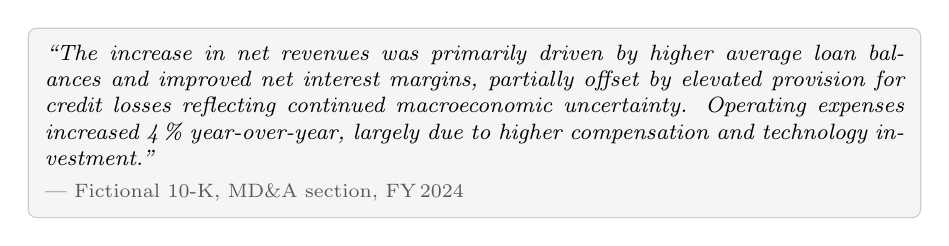
\begin{tikzpicture}
\node[draw=gray!40, fill=SoftGray, rounded corners=3pt,
      text width=0.90\linewidth, inner sep=6pt,
      font=\footnotesize\itshape, align=justify] {
``The increase in net revenues was primarily driven by higher average
loan balances and improved net interest margins, partially offset by
elevated provision for credit losses reflecting continued macroeconomic
uncertainty. Operating expenses increased 4\,\% year-over-year,
largely due to higher compensation and technology investment.''
\vspace{2pt}\\
\upshape\textcolor{gray!70!black}{\scriptsize --- Fictional 10-K, MD\&A section, FY\,2024}
};
\end{tikzpicture}
\end{block}
\end{column}

% ── right: earnings call transcript ─────────────────────────
\begin{column}{0.47\textwidth}
\begin{block}{Example 2 --- Earnings call transcript}
Spoken language converted to text. Rich in hedging, forward-looking
statements, and analyst questions. No labels attached.

\vspace{0.12cm}
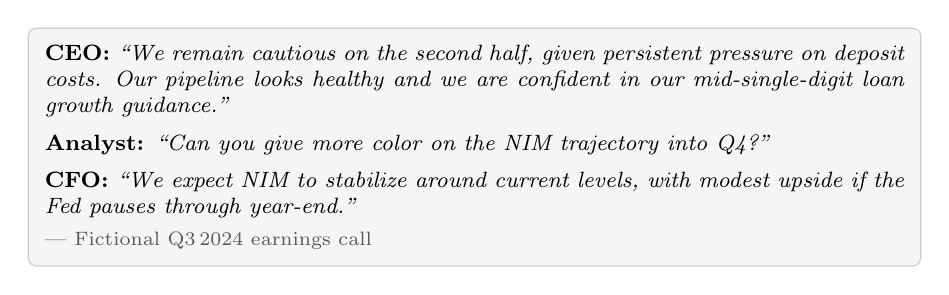
\begin{tikzpicture}
\node[draw=gray!40, fill=SoftGray, rounded corners=3pt,
      text width=0.90\linewidth, inner sep=6pt,
      font=\footnotesize, align=justify] {
\textbf{CEO:} \textit{``We remain cautious on the second half, given
persistent pressure on deposit costs. Our pipeline looks healthy and
we are confident in our mid-single-digit loan growth guidance.''}\\[4pt]
\textbf{Analyst:} \textit{``Can you give more color on the NIM
trajectory into Q4?''}\\[4pt]
\textbf{CFO:} \textit{``We expect NIM to stabilize around current
levels, with modest upside if the Fed pauses through year-end.''}
\vspace{2pt}\\
\textcolor{gray!70!black}{\scriptsize --- Fictional Q3\,2024 earnings call}
};
\end{tikzpicture}
\end{block}
\end{column}

\end{columns}
\end{frame}
%
%..................................................................
%
\begin{frame}{Why Domain Matters}
\begin{itemize}
    \item Language is deeply contextual.
    \item The same word can play very different semantic roles across domains.
    \item In finance, a \textit{spread} is not the same thing as in epidemiology or in cooking.
    \item The word \textit{bank} may refer to a financial institution, a river bank, a mine bank, or a billiard cushion.
\end{itemize}

\vspace{0.15cm}
\begin{alertblock}{Domain-specific corpora}
Working with domain-specific corpora reduces ambiguity, narrows the prediction space, and often produces more intelligible and more robust models.
\end{alertblock}
\end{frame}
%
%..................................................................
%
\begin{frame}{Where Do Text Corpora Come From?}
Typical sources of textual corpora include:
\begin{itemize}
    \item web pages and news feeds;
    \item PDF reports, filings, contracts, and manuals;
    \item emails, chats, tickets, and CRM interactions;
    \item social media posts and comments;
    \item structured databases with textual fields;
    \item speech transcripts and meeting notes.
\end{itemize}

\vspace{0.15cm}
%\begin{block}{A practical remark}
%APIs are usually preferable to scraping whenever they are available. Scraping may still be needed, but it is only one component of a modern document pipeline.
%\end{block}
\end{frame}
%
%..................................................................
%
\begin{frame}{Preprocessing Is Not Neutral}
Preprocessing is often introduced as a standard pipeline, but in practice it depends on the task.

\vspace{0.15cm}
\begin{columns}[T]
\begin{column}{0.48\textwidth}
\begin{block}{Typical operations}
\begin{itemize}
    \item tokenization
    \item lowercasing
    \item punctuation removal
    \item stop-word removal
    \item stemming
    \item lemmatization
\end{itemize}
\end{block}
\end{column}
\begin{column}{0.48\textwidth}
\begin{block}{Why caution is needed}
\begin{itemize}
    \item numbers may carry signal;
    \item punctuation may encode structure;
    \item stop-words may affect sentiment;
    \item case may matter for names and entities.
\end{itemize}
\end{block}
\end{column}
\end{columns}
\end{frame}
%
%..................................................................
%
\begin{frame}{Tokenization}
\begin{itemize}
    \item Tokenization is the process of segmenting text into smaller units called \textbf{tokens}.
    \item Tokens may be words, subwords, characters, or even punctuation symbols depending on the representation model.
    \item In classical NLP, tokenization typically splits text into sentences and words.
\end{itemize}

\vspace{0.2cm}
\begin{block}{Example}
Text: \texttt{The cat sat on the mat.}
\[
\text{Tokens} = (\texttt{the},\texttt{cat},\texttt{sat},\texttt{on},\texttt{the},\texttt{mat},\texttt{.})
\]
\end{block}
\end{frame}
%
%..................................................................
%
\begin{frame}{Beyond Word Boundaries: Subword Tokenization}
Classical tokenization produces word-level tokens by splitting on whitespace and punctuation.
Two structural problems arise immediately:
\vspace{0.5cm}
\begin{itemize}
    \item \textbf{Out-of-vocabulary (OOV) words}: rare or technical terms unseen during training
    are reduced to a generic \texttt{[UNK]} token, losing all information.
\vspace{0.5cm}
    \item \textbf{Vocabulary explosion}: inflected and compound forms generate many distinct
    dictionary entries.
\end{itemize}
\end{frame} 
%
%..................................................................
%
\begin{frame}{Beyond Word Boundaries: Subword Tokenization}
\vspace{0.15cm}
\begin{block}{Financial text is particularly affected}
Terms such as \texttt{non-performing}, \texttt{EBITDA}, or \texttt{rebalancing} are rare
in general corpora and are frequently classified as unknown by word-level tokenizers.
\end{block}
 
\vspace{0.15cm}
\begin{alertblock}{The response: subword tokenization}
Split words into reusable fragments. Any word can be decomposed into known pieces --
at worst into individual characters -- while keeping the vocabulary small and fixed.
\end{alertblock}
\end{frame}
%
%..................................................................
%
\begin{frame}{Subword Tokenization: BPE, WordPiece, SentencePiece}
\begin{columns}[T]
\begin{column}{0.50\textwidth}
\begin{block}{Byte Pair Encoding (BPE)}
Start from characters. Iteratively merge the most frequent adjacent symbol pair
until the target vocabulary size is reached.
\[
\texttt{under} \;|\; \texttt{val} \;|\; \texttt{uation}
\]
GPT-2 and GPT-4 use BPE with $\sim$50\,000 tokens.
\end{block}
\end{column}
\begin{column}{0.46\textwidth}
\begin{block}{Variants in practice}
\begin{itemize}
    \item \textbf{WordPiece} (BERT): non-initial fragments prefixed with \texttt{\#\#}.
    \item \textbf{SentencePiece}: language-agnostic; treats raw bytes.
    \item \textbf{Unigram LM} (XLNet): probabilistic segmentation.
\end{itemize}
\end{block}
\end{column}
\end{columns}
 
\vspace{0.15cm}
\begin{alertblock}{Forward reference -- Lesson 3}
Every transformer model uses subword tokenization. The tokenizer choice shapes
how financial terms, tickers, and numeric expressions enter the model.
\end{alertblock}
\end{frame}
%
%..................................................................
%
\begin{frame}{BPE: The main idea}
\begin{block}{Byte Pair Encoding}
BPE builds a vocabulary of frequent \textbf{character sequences} by repeatedly merging the \textbf{most common adjacent pair} in the training data.
\end{block}

\vspace{0.3cm}
\textbf{Very simple workflow}
\begin{enumerate}
  \item Start from characters (or bytes).
  \item Count all adjacent pairs.
  \item Merge the most frequent pair into a new symbol.
  \item Repeat many times.
\end{enumerate}

\vspace{0.3cm}
At the end, words are represented as a sequence of learned pieces such as:
\[
\texttt{lower} = \texttt{low} + \texttt{er}
\]
\end{frame}
%
%..................................................................
%
\begin{frame}{BPE: The main idea}
Suppose our training corpus contains these words:
\begin{center}
\texttt{low}, \texttt{lower}, \texttt{lowest}, \texttt{newer}
\end{center}

Initially we split every word into characters:
\begin{align*}
\texttt{low} &\rightarrow \texttt{l\; o\; w}\\
\texttt{lower} &\rightarrow \texttt{l\; o\; w\; e\; r}\\
\texttt{lowest} &\rightarrow \texttt{l\; o\; w\; e\; s\; t}\\
\texttt{newer} &\rightarrow \texttt{n\; e\; w\; e\; r}
\end{align*}

\vspace{0.2cm}
Now we count adjacent pairs such as:
\texttt{(l,o)}, \texttt{(o,w)}, \texttt{(w,e)}, \texttt{(e,r)}, \texttt{(e,s)}.
\end{frame}
%
%..................................................................
%
\begin{frame}{BPE: The main idea}
Assume the most frequent pairs are found in this order.

\begin{center}
\begin{tabular}{@{}>{\ttfamily}l l@{}}
\toprule
Merge & Interpretation \\
\midrule
l o $\rightarrow$ lo & create token \texttt{lo} \\
o w $\rightarrow$ ow & create token \texttt{ow} \\
lo w $\rightarrow$ low & create token \texttt{low} \\
e r $\rightarrow$ er & create token \texttt{er} \\
e s t $\rightarrow$ est & create token \texttt{est} \\
\bottomrule
\end{tabular}
\end{center}

\vspace{0.3cm}
Then some words can be encoded as:
\begin{align*}
\texttt{lower} &\rightarrow \texttt{low + er}\\
\texttt{lowest} &\rightarrow \texttt{low + est}\\
\texttt{newer} &\rightarrow \texttt{n + ew + er} \quad \text{or similar, depending on learned merges}
\end{align*}
\end{frame}
%
%..................................................................
%
\begin{frame}{Tokenization of Financial Text: A Concrete Example}

How does a BPE tokenizer (GPT-4 class) segment typical financial inputs?

\vspace{0.15cm}
\begin{center}
\renewcommand{\arraystretch}{1.35}
\begin{tabular}{>{\raggedright\arraybackslash}p{0.30\linewidth}
                >{\ttfamily\raggedright\arraybackslash}p{0.58\linewidth}}
\toprule
\textbf{Input} & \textbf{Subword tokens} \\
\midrule
\texttt{AAPL}           & AA | PL \\
\texttt{\$12,345.67}    & \$ | 12 | , | 345 | . | 67 \\
\texttt{non-performing} & non | - | performing \\
\texttt{10-K}           & 10 | - | K \\
\texttt{EBITDA}         & EB | IT | DA \\
\texttt{rebalancing}    & re | bal | ancing \\
\bottomrule
\end{tabular}
\end{center}
\end{frame}
%
%..................................................................
%
\begin{frame}{Tokenization of Financial Text: A Concrete Example}
\vspace{0.12cm}
\begin{alertblock}{Why this matters for finance}
Numbers are split into arbitrary fragments, destroying their numerical meaning.
Tickers and acronyms are decomposed into semantically meaningless pieces.
This is one reason why LLMs struggle with arithmetic and precise entity matching
--- a theme we revisit in Lessons~3 and~5.
\end{alertblock}
\end{frame}
%
%..................................................................
%
\begin{frame}{Stop Words: Helpful or Dangerous?}
\begin{itemize}
    \item Stop words are highly frequent terms that often carry limited discriminative power.
    \item Examples in English include words such as \textbf{the}, \textbf{and}, \textbf{to}, \textbf{of}.
    \item Removing them can reduce noise and dimensionality, but it may also delete relevant information.
\end{itemize}

\vspace{0.15cm}
\begin{alertblock}{There is no universal stop-word list}
In sentiment analysis, removing \textbf{not} may completely alter the polarity of a sentence. In legal or financial documents, frequent function words may contribute to structure and meaning.
\end{alertblock}
\end{frame}
%
%..................................................................
%
\begin{frame}{Stemming and Lemmatization}
\begin{columns}[T]
\begin{column}{0.52\textwidth}
\begin{block}{Stemming}
A heuristic reduction of words to a crude root by removing prefixes or suffixes.
\[
\texttt{helpful} \rightarrow \texttt{help}
\]
Stemming is fast, but the result is not always a valid word.
\end{block}
\end{column}
\begin{column}{0.44\textwidth}
\begin{block}{Lemmatization}
A linguistically informed reduction to the canonical form (lemma):
\[
\texttt{was} \rightarrow \texttt{be}
\]
It is usually cleaner, but it requires more linguistic knowledge.
\end{block}
\end{column}
\end{columns}

\vspace{0.15cm}
\begin{block}{Task dependence}
For retrieval, stemming or lemmatization may increase recall. For generation or high-fidelity parsing, aggressive normalization may remove useful distinctions.
\end{block}
\end{frame}
%
%..................................................................
%
\begin{frame}{Stemming and Lemmatization}
	\begin{itemize}
		\item Lemmatization resolves words to their dictionary form (known as lemma) for which it requires detailed dictionaries in which the algorithm can look into and link words to their corresponding lemmas.
		\item For example, the words \textbf{running }, \textbf{ runs }  and  \textbf{ ran }  are all forms of the word \textbf{ run }, so \textbf{ run} is the lemma of all the previous words.
	\end{itemize}
	\begin{center}
	
\includegraphics[scale=0.5]{../05-pictures/chapter-01_pic_0.png}
	\end{center}
\end{frame}
%
%..................................................................
%
\begin{frame}{A Minimal Classical Pipeline}
\begin{center}
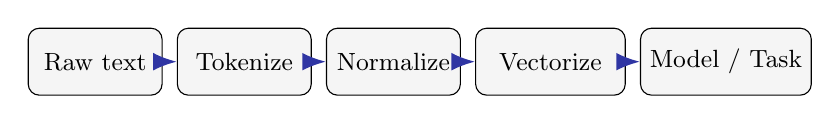
\begin{tikzpicture}[node distance=0.35cm and 0.18cm, every node/.style={font=\small}]
\node[draw, rounded corners, fill=SoftGray, minimum width=1.7cm, minimum height=0.85cm] (a) {Raw text};
\node[draw, rounded corners, fill=SoftGray, right=of a, minimum width=1.7cm, minimum height=0.85cm] (b) {Tokenize};
\node[draw, rounded corners, fill=SoftGray, right=of b, minimum width=1.7cm, minimum height=0.85cm] (c) {Normalize};
\node[draw, rounded corners, fill=SoftGray, right=of c, minimum width=1.9cm, minimum height=0.85cm] (d) {Vectorize};
\node[draw, rounded corners, fill=SoftGray, right=of d, minimum width=2.0cm, minimum height=0.85cm] (e) {Model / Task};
\draw[-{Latex[length=3mm]}, thick, CourseBlue] (a) -- (b);
\draw[-{Latex[length=3mm]}, thick, CourseBlue] (b) -- (c);
\draw[-{Latex[length=3mm]}, thick, CourseBlue] (c) -- (d);
\draw[-{Latex[length=3mm]}, thick, CourseBlue] (d) -- (e);
\end{tikzpicture}
\end{center}

\vspace{0.15cm}
\begin{block}{What changes across paradigms?}
The early stages remain recognizable even today, but the \textbf{vectorize} block changes radically when we move from sparse counts to embeddings and then to contextual representations.
\end{block}
\end{frame}
%__________________________________________________________________________
%
\section{Sparse Vector Representations of Text}
%__________________________________________________________________________
%
\begin{frame}{The Representation Problem}
Machine learning algorithms operate in a numerical feature space. Therefore, before we can train or compare models on text, we must transform documents into vectors.

\vspace{0.15cm}
\begin{block}{Core question}
Given a document $d$, what should the vector $\vect{x}(d)$ contain?
\end{block}

\vspace{0.15cm}
Three fundamental ideas dominated early NLP:
\begin{itemize}
    \item represent a document through the words it contains;
    \item assign numerical weights to those words;
    \item define similarity or distance in the resulting vector space.
\end{itemize}
\end{frame}
%
%..................................................................
%
\begin{frame}{Bag-of-Words: The Simplest Encoding}
In a \textbf{bag-of-words} model, each document is represented as a vector whose length equals the vocabulary size of the corpus.

\vspace{0.15cm}
\begin{block}{Vocabulary}
If the corpus vocabulary is
\[
V = (w_1,w_2,\dots,w_{|V|}),
\]
then each document $d$ is mapped to a vector in $\R^{|V|}$.
\end{block}

\vspace{0.1cm}
\begin{alertblock}{What is ignored?}
Bag-of-words ignores word order. It assumes that meaning is encoded primarily in vocabulary rather than in sequence.
\end{alertblock}
\end{frame}
%
%..................................................................
%
\begin{frame}{Bag-of-Words: The Simplest Encoding}
Suppose we have the three short documents:
\begin{align*}
 d_1 &: \texttt{low interest rates usually mean low interest income}\\
 d_2 &: \texttt{banks lend money because money must create value}\\
 d_3 &: \texttt{banks provide credit because people need money}
\end{align*}

A possible vocabulary is:

\[
\begin{aligned}
V = (&\texttt{banks},\texttt{because},\texttt{create},\texttt{credit},\texttt{income},\texttt{interest},\texttt{lend},\texttt{low},\texttt{mean},\texttt{money},\\
     &\texttt{must},\texttt{need},\texttt{people},\texttt{provide},\texttt{rates},\texttt{usually},\texttt{value})
\end{aligned}
\]

The corpus can then be represented as a \textbf{document-term matrix} where rows are documents and columns are vocabulary items.
\end{frame}
%
%..................................................................
%
\begin{frame}{Bag-of-Words: The Simplest Encoding}
\centering

\includegraphics[scale=.45]{../05-pictures/chapter-01_pic_1.png} 
\end{frame}
%
%..................................................................
%
\begin{frame}{Count Vectors}
The simplest bag-of-words encoding is the \textbf{count vector}:
\[
\vect{x}(d) = (c_1,c_2,\dots,c_{|V|}),
\]
where $c_j$ is the number of occurrences of word $w_j$ in document $d$.

\vspace{0.15cm}
\begin{block}{Example}
If
\[
V=(\texttt{market},\texttt{rises},\texttt{falls}),
\]
and the document is
\[
 d = \texttt{market rises market},
\]
then
\[
\vect{x}(d) = (2,1,0).
\]
\end{block}
\end{frame}
%
%..................................................................
%
\begin{frame}{Bag-of-Words: The Simplest Encoding}
\centering
\only<1>{
\includegraphics[scale=.45]{../05-pictures/chapter-01_pic_2.png}}%
\only<2>{
\includegraphics[scale=.45]{../05-pictures/chapter-01_pic_3.png}}%
\only<3>{
\includegraphics[scale=.45]{../05-pictures/chapter-01_pic_4.png}}
\end{frame}
%
%..................................................................
%
\begin{frame}{Beyond Single Words: N-grams}
The bag-of-words model discards word order entirely.
Two sentences with identical vocabulary but different arrangement receive identical representations.
 
\vspace{0.12cm}
\begin{block}{A financial counterexample}
\begin{center}
\texttt{the fund buy the bank} \quad $\neq$ \quad \texttt{the bank buy the fund}
\end{center}
Identical unigram counts; very different meaning in practice.
\end{block}
 
\vspace{0.12cm}
An \textbf{$n$-gram} is a contiguous sequence of $n$ tokens.
Extending the feature space to sequences of length $n$:
\begin{center}
\small
\begin{tabular}{lll}
\toprule
$n$ & Name & Financial example \\
\midrule
1 & unigram & \texttt{rate}, \texttt{cut}, \texttt{yield} \\
2 & bigram  & \texttt{interest rate}, \texttt{yield curve} \\
3 & trigram & \texttt{central bank policy} \\
\bottomrule
\end{tabular}
\end{center}
\end{frame}
%
%..................................................................
%
\begin{frame}{N-grams: Local Power and Global Sparsity}
\begin{columns}[T]
\begin{column}{0.48\textwidth}
\begin{block}{What n-grams capture}
\begin{itemize}
    \item Local word order and fixed phrases.
    \item Negation: \texttt{no default}, \texttt{not profitable}.
    \item Domain collocations:\\ \texttt{yield curve}, \texttt{central bank}.
    \item Sentiment units:\\ \texttt{strong growth}, \texttt{sharp decline}.
\end{itemize}
\end{block}
\end{column}
\begin{column}{0.48\textwidth}
\begin{block}{The sparsity cost}
A bigram vocabulary has up to $|V|^2$ entries.
In practice:
\begin{itemize}
    \item most bigrams are absent from any given document;
    \item the feature matrix becomes far sparser;
    \item memory and compute grow fast with $n$.
\end{itemize}
\end{block}
\end{column}
\end{columns}
 
\vspace{0.18cm}
\begin{alertblock}{The fundamental tension}
N-grams improve local context modelling but the vocabulary explosion and worsening sparsity
limit their scalability. This is one of the motivations for learned dense representations.
\end{alertblock}
\end{frame}
%
%..................................................................
%
\begin{frame}{One-Hot Encoding}
A related but even simpler encoding is \textbf{one-hot} or \textbf{binary} encoding:
\[
 x_j(d)=
 \begin{cases}
 1 & \text{if } w_j \text{ appears in } d,\\
 0 & \text{otherwise.}
 \end{cases}
\]

\vspace{0.15cm}
\begin{block}{Interpretation}
Count vectors retain multiplicity; one-hot vectors only retain presence or absence.
\end{block}

\vspace{0.15cm}
\begin{alertblock}{Why we do not dwell on it today}
One-hot is conceptually useful, but in modern NLP it is mostly a stepping stone toward richer representations.
\end{alertblock}
\end{frame}
%
%..................................................................
%
\begin{frame}{Term Frequency (TF)}
Raw counts are affected by document length. Longer documents tend to have larger counts even if they are not more informative.

\vspace{0.15cm}
A normalized alternative is \textbf{term frequency}:
\[
\mathrm{tf}(t,d) = \frac{\#(t \text{ in } d)}{\text{total number of tokens in } d}.
\]

\vspace{0.15cm}
\begin{block}{Interpretation}
TF measures how important a term is \emph{within a specific document}, relative to that document's length.
\end{block}
\end{frame}
%
%..................................................................
%
\begin{frame}{Inverse Document Frequency (IDF)}
Some words are frequent in almost every document and therefore carry little discriminative power.

\vspace{0.15cm}
The \textbf{inverse document frequency} of term $t$ in corpus $D$ is:
\[
\mathrm{idf}(t,D) = \log\frac{N}{|\{d\in D : t\in d\}|},
\]
where:
\begin{itemize}
    \item $N$ is the number of documents in the corpus;
    \item the denominator counts how many documents contain term $t$.
\end{itemize}

\vspace{0.1cm}
Rare terms have high IDF; ubiquitous terms have low IDF.
\end{frame}
%
%..................................................................
%
\begin{frame}{TF--IDF}
The most famous classical weighting scheme is:
\[
\mathrm{tfidf}(t,d,D)=\mathrm{tf}(t,d)\cdot\mathrm{idf}(t,D).
\]

\vspace{0.15cm}
\begin{block}{Why it works}
TF--IDF rewards words that are frequent in a given document but not too frequent in the corpus as a whole.
\end{block}

\vspace{0.12cm}
\begin{itemize}
    \item High TF alone may privilege long documents.
    \item High IDF alone may privilege rare but irrelevant words.
    \item Their product is a practical compromise for feature weighting.
\end{itemize}
\end{frame}
%
%..................................................................
%
\begin{frame}{TF--IDF}
\centering
\only<1>{
\includegraphics[scale=.45]{../05-pictures/chapter-01_pic_5.png}}%
\only<2>{
\includegraphics[scale=.45]{../05-pictures/chapter-01_pic_6.png}}%
\only<3>{
\includegraphics[scale=.45]{../05-pictures/chapter-01_pic_7.png}}
\end{frame}
%
%..................................................................
%
\begin{frame}{A Small TF--IDF Intuition}
Suppose the term "\textbf{merger}" appears often in one specific financial news article, but only in a small fraction of the corpus.

\vspace{0.15cm}
Then:
\begin{itemize}
    \item its \textbf{TF} is high in that article;
    \item its \textbf{IDF} is also relatively high in the corpus;
    \item hence its TF--IDF weight becomes large.
\end{itemize}

\vspace{0.15cm}
By contrast, a term such as "\textbf{the}" may have high TF in many documents, but its IDF is tiny because it appears everywhere.
\end{frame}
%
%..................................................................
%
\begin{frame}{A Worked Example: TF--IDF}

Consider a corpus of $N=3$ documents with vocabulary
$V = \{\texttt{rate},\,\texttt{cut},\,\texttt{bond}\}$:

\vspace{0.08cm}
\begin{center}
\renewcommand{\arraystretch}{1.2}
\begin{tabular}{lccc|ccc}
\toprule
 & \multicolumn{3}{c|}{\textbf{Raw count}} & \multicolumn{3}{c}{\textbf{TF--IDF weight}} \\
 & rate & cut & bond & rate & cut & bond \\
\midrule
$d_1$: \textit{rate cut rate} & 2 & 1 & 0 & $2\!\times\!0 = 0$ & $1\!\times\!0.41 = 0.41$ & 0 \\
$d_2$: \textit{bond rate bond} & 1 & 0 & 2 & $1\!\times\!0 = 0$ & 0 & $2\!\times\!0.41 = 0.81$ \\
$d_3$: \textit{rate bond cut} & 1 & 1 & 1 & $1\!\times\!0 = 0$ & $1\!\times\!0.41 = 0.41$ & $1\!\times\!0.41 = 0.41$ \\
\bottomrule
\end{tabular}
\end{center}
{Using $\mathrm{idf}(t)=\ln(N/\mathrm{df}(t))$:
\texttt{rate} appears in all 3 docs $\Rightarrow \ln(3/3)=0$;
\texttt{cut} and \texttt{bond} each in 2 docs $\Rightarrow \ln(3/2)\approx 0.41$.
Note: \texttt{rate} vanishes entirely --- a word present in \emph{every} document has zero
discriminative value under TF--IDF.}

\end{frame}
%
%..................................................................
%
\begin{frame}{Measuring Similarity Between Documents}

We now have a way to represent every document as a numerical vector
(BoW counts or TF--IDF weights).  A spontaneous question arises:

\begin{tcolorbox}[colback=blue!5!white, colframe=blue!75!black,
  title=\textbf{The core question}]
Given two document vectors $\mathbf{x}$ and $\mathbf{y}$
in $\mathbb{R}^{|V|}$, how do we quantify
\emph{how similar} they are?
\end{tcolorbox}

\medskip
This is not just an abstract question---it has immediate practical
applications:

\begin{itemize}
\item \textbf{Search:} given a user query, find the most similar
      documents in a corpus.
\item \textbf{Clustering:} group together documents that discuss
      similar topics.
\item \textbf{Duplicate detection:} identify near-copies of
      financial filings or news articles.
\item \textbf{Recommendation:} suggest articles similar to ones
      a user has already read.
\end{itemize}

\end{frame}
%
%..................................................................
%
\begin{frame}{A First Attempt: Euclidean Distance}

The most familiar distance measure is the Euclidean distance:
\[
  d(\mathbf{x}, \mathbf{y})
  \;=\;
  \|\mathbf{x} - \mathbf{y}\|
  \;=\;
  \sqrt{\sum_{i=1}^{|V|} (x_i - y_i)^2}\,.
\]
\end{frame}
%
%..................................................................
%
\begin{frame}{A First Attempt: Euclidean Distance}
\textbf{But it has a serious problem with text vectors.}

\begin{columns}[T]
\begin{column}{0.55\textwidth}

\bigskip

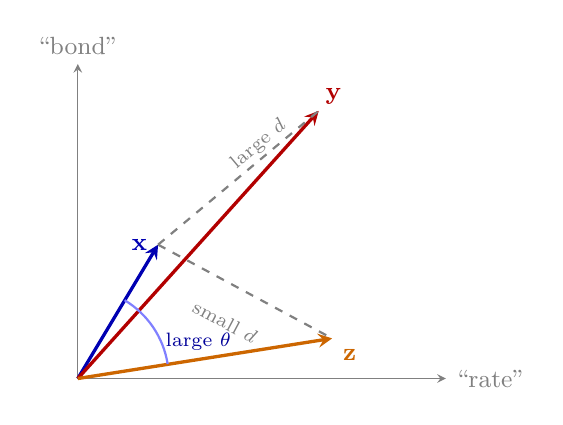
\begin{tikzpicture}[scale=0.85, >=stealth]
  % axes
  \draw[->, gray] (0,0) -- (5.5,0) node[right, font=\small] {``rate''};
  \draw[->, gray] (0,0) -- (0,4.7) node[above, font=\small] {``bond''};

  % Short doc about bonds+rates
  \draw[->, very thick, blue!70!black] (0,0) -- (1.2, 2.0)
    node[left, font=\small\bfseries, text=blue!70!black] {$\mathbf{x}$};
  % Long doc -- same topic, same direction, 3x longer
  \draw[->, very thick, red!70!black] (0,0) -- (3.6, 4.0)
    node[above right=-2pt, font=\small\bfseries, text=red!70!black]
    {$\mathbf{y}$};
  % Different topic doc -- mostly "rate", very little "bond"
  \draw[->, very thick, orange!80!black] (0,0) -- (3.8, 0.6)
    node[below right, font=\small\bfseries, text=orange!80!black]
    {$\mathbf{z}$};

  % Euclidean distance line x--y (large)
  \draw[dashed, thick, gray] (1.2, 2.0) -- (3.6, 4.0);
  \node[font=\scriptsize, gray, rotate=40] at (2.7, 3.5) {large $d$};

  % Euclidean distance line x--z (shorter!)
  \draw[dashed, thick, gray] (1.2, 2.0) -- (3.8, 0.6);
  \node[font=\scriptsize, gray, rotate=-28] at (2.2, 0.85) {small $d$};

  % angle arc between x-direction and z-direction (large angle)
  \draw[blue!50, thick] (0.7, 1.17)
    arc[start angle=59, end angle=9, radius=1.36];
  \node[font=\scriptsize, blue!60!black] at (1.8, 0.55) {large $\theta$};
\end{tikzpicture}
\end{column}

\begin{column}{0.43\textwidth}

\vspace{-0.3cm}
\begin{tcolorbox}[colback=red!5!white, colframe=red!70!black,
  title=\textbf{The magnitude trap}]
$\mathbf{x}$ is a \emph{short} article about bonds and rates.\\[3pt]
$\mathbf{y}$ is a \emph{long} article about the \emph{same} topic
--- all TF--IDF weights are simply larger.\\[3pt]
$\mathbf{z}$ is about a \emph{different} topic entirely.\\[6pt]
Euclidean distance says $\mathbf{x}$ is closer to $\mathbf{z}$
than to $\mathbf{y}$, even though $\mathbf{x}$ and $\mathbf{y}$
discuss the same subject!
\end{tcolorbox}

%\medskip
%{\small The problem: Euclidean distance conflates
%\textbf{what} a document is about (direction)
%with \textbf{how long} it is (magnitude).}
\end{column}
\end{columns}

\end{frame}
%
%..................................................................
%
\begin{frame}{Cosine Similarity: Comparing Directions, Not Magnitudes}

The fix is simple: ignore the length of the vectors and compare
only their \textbf{directions}.

\[
  \boxed{\;
  \cos(\mathbf{x},\, \mathbf{y})
  \;=\;
  \frac{\mathbf{x}^{\!\top} \mathbf{y}}
       {\|\mathbf{x}\|\;\|\mathbf{y}\|}
  \;=\;
  \frac{\displaystyle\sum_{i=1}^{|V|} x_i \, y_i}
       {\displaystyle\sqrt{\sum_i x_i^2}\;\sqrt{\sum_i y_i^2}}
  \;}
\]
\end{frame}
%
%..................................................................
%
\begin{frame}{Cosine Similarity: Comparing Directions, Not Magnitudes}

\begin{columns}[T]
\begin{column}{0.48\textwidth}
\begin{tcolorbox}[colback=green!5!white, colframe=green!60!black,
  title=\textbf{Geometric intuition}]
Cosine similarity $=$ the cosine of the \textbf{angle}~$\theta$
between the two vectors.\\[6pt]
\begin{tabular}{rl}
$\cos\theta = 1$  & $\Rightarrow$ identical direction \\
$\cos\theta = 0$  & $\Rightarrow$ orthogonal (no overlap) \\
$\cos\theta = -1$ & $\Rightarrow$ opposite directions \\
\end{tabular}\\[6pt]
{\small (For TF--IDF vectors, all weights $\geq 0$,
so $\cos\theta \in [0,\,1]$.)}
\end{tcolorbox}
\end{column}

\begin{column}{0.48\textwidth}
\begin{tcolorbox}[colback=blue!5!white, colframe=blue!75!black,
  title=\textbf{Why this solves the problem}]
\begin{itemize}
\item Dividing by $\|\mathbf{x}\|$ and $\|\mathbf{y}\|$
      \textbf{normalizes out} the effect of document length.
\item A short article and a long article on the
      \emph{same} topic will point in the
      \emph{same} direction $\Rightarrow$ $\cos\theta \approx 1$.
\item Two articles on \emph{different} topics
      will point in different directions $\Rightarrow$ $\cos\theta \approx 0$.
\end{itemize}
\end{tcolorbox}
\end{column}
\end{columns}

\end{frame}
%
%..................................................................
%
\begin{frame}{Worked Example: Cosine Similarity}
\small
Using the TF--IDF vectors from the previous example
(vocabulary: \{rate, cut, bond\}):

\begin{center}
\renewcommand{\arraystretch}{1.3}
\begin{tabular}{l c c c}
\hline
         & rate & cut & bond \\
\hline
$d_1$    & 0    & 0.41 & 0    \\
$d_2$    & 0    & 0    & 0.81 \\
$d_3$    & 0    & 0.41 & 0.41 \\
\hline
\end{tabular}
\end{center}


\textbf{Compute} $\cos(d_1, d_3)$:
\[
  \cos(d_1, d_3)
  = \frac{(0)(0) + (0.41)(0.41) + (0)(0.41)}
         {\sqrt{0^2 + 0.41^2 + 0^2}\;\sqrt{0^2 + 0.41^2 + 0.41^2}}
  = \frac{0.168}{0.41 \times 0.58}
  \approx \mathbf{0.707}
\]

\textbf{Compute} $\cos(d_1, d_2)$:
\[
  \cos(d_1, d_2)
  = \frac{(0)(0) + (0.41)(0) + (0)(0.81)}
         {0.41 \times 0.81}
  = \frac{0}{0.33}
  = \mathbf{0}
\]
\end{frame}
%
%..................................................................
%
\begin{frame}{A Simple Vector-Space Picture}

\begin{center}
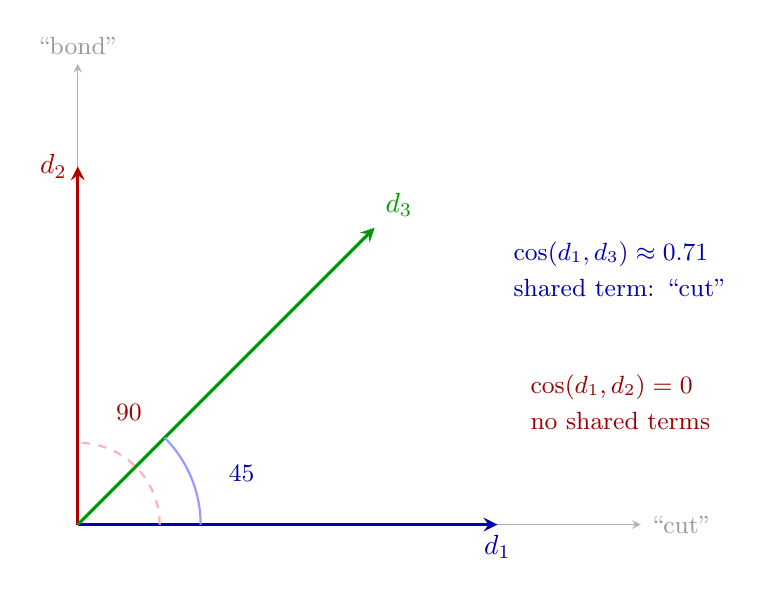
\begin{tikzpicture}[scale=1.3, >=stealth]
  % axes
  \draw[->, gray!60] (0,0) -- (5.5,0)
    node[right, font=\small, gray!80] {``cut''};
  \draw[->, gray!60] (0,0) -- (0,4.5)
    node[above, font=\small, gray!80] {``bond''};

  % d1: (0.41, 0) -- only "cut"
  \draw[->, very thick, blue!70!black] (0,0) -- (4.1, 0)
    node[below, font=\bfseries, text=blue!70!black] {$d_1$};

  % d2: (0, 0.81) -- only "bond"
  \draw[->, very thick, red!70!black] (0,0) -- (0, 3.5)
    node[left, font=\bfseries, text=red!70!black] {$d_2$};

  % d3: (0.41, 0.41) -- both
  \draw[->, very thick, green!60!black] (0,0) -- (2.9, 2.9)
    node[above right, font=\bfseries, text=green!60!black] {$d_3$};

  % angle between d1 and d3
  \draw[blue!40, thick] (1.2, 0) arc[start angle=0, end angle=45, radius=1.2];
  \node[font=\small, blue!60!black] at (1.6, 0.5) {$45°$};

  % angle between d1 and d2
  \draw[red!30, thick, dashed] (0.8, 0) arc[start angle=0, end angle=90, radius=0.8];
  \node[font=\small, red!60!black] at (0.5, 1.1) {$90°$};

  % annotations
  \node[font=\small, align=left, text=blue!70!black] at (5.3, 2.5)
    {$\cos(d_1, d_3) \approx 0.71$\\[2pt] shared term: ``cut''};
  \node[font=\small, align=left, text=red!60!black] at (5.3, 1.2)
    {$\cos(d_1, d_2) = 0$\\[2pt] no shared terms};
\end{tikzpicture}
\end{center}

\medskip

\begin{itemize}
\item Documents that share terms point in \textbf{similar directions}
      $\Rightarrow$ high cosine similarity.
\item Documents with no common terms are \textbf{orthogonal}
      $\Rightarrow$ zero cosine similarity.
\item The \textbf{angle} between vectors, not their length, determines
      similarity.
\end{itemize}

\end{frame}
%
%..................................................................
%
\begin{frame}{From Feature Weighting to Document Retrieval}
 
So far we have used TF--IDF as a \textbf{feature-weighting} scheme:
given a fixed corpus, assign each term in each document a numeric weight
that captures how \emph{important} that term is for that document.
 
\medskip
But TF--IDF vectors enable a second, very practical task:
 
\begin{tcolorbox}[colback=blue!5!white, colframe=blue!75!black,
  title=\textbf{Text Retrieval (a.k.a.\ Information Retrieval)}]
Given a collection of $N$ documents and a short user
\textbf{query}~$q$ (e.g.\ a few keywords), \emph{rank} the documents
from most relevant to least relevant with respect to~$q$.
\end{tcolorbox}
 
\medskip
\textbf{Examples in finance:}
\begin{itemize}
\item Search ``\texttt{interest rate hike}'' across 50\,000 analyst reports.
\item Find the SEC filings most relevant to ``\texttt{credit default swap}''.
\item A RAG pipeline retrieves context passages before prompting an LLM.
\end{itemize}
 
\end{frame}
%
%..................................................................
%
\begin{frame}{How TF--IDF Retrieval Works}
 
\begin{enumerate}
\item \textbf{Index Phase.} Represent every document $d_j$ as a TF--IDF
      vector $\mathbf{v}_j \in \mathbb{R}^{|V|}$.
\item \textbf{Query Phase.} Represent the query $q$ as a (very sparse)
      TF--IDF vector $\mathbf{v}_q$ using the \emph{same} vocabulary.
\item \textbf{Scoring.} Rank documents by similarity, typically
      \textbf{cosine similarity}:
\[
  \text{score}(q,\, d_j)
  \;=\;
  \cos(\mathbf{v}_q,\, \mathbf{v}_j)
  \;=\;
  \frac{\mathbf{v}_q \cdot \mathbf{v}_j}
       {\|\mathbf{v}_q\|\;\|\mathbf{v}_j\|}\,.
\]
\item \textbf{Return} the top-$k$ documents with the highest scores.
\end{enumerate}
 
\medskip
\begin{tcolorbox}[colback=gray!8, colframe=gray!60,
  title=\textbf{Key idea}]
The query is just another ``document''---a very short one.
We compare its vector against every document vector in the corpus
and return the closest matches.
\end{tcolorbox}
 
\end{frame}
%
%..................................................................
%
\begin{frame}{A Concrete Retrieval Example}
 
\textbf{Corpus:} three financial news articles.\\[2pt]
\textbf{Query:} \texttt{``interest rate''}
 
\bigskip
 
\begin{center}
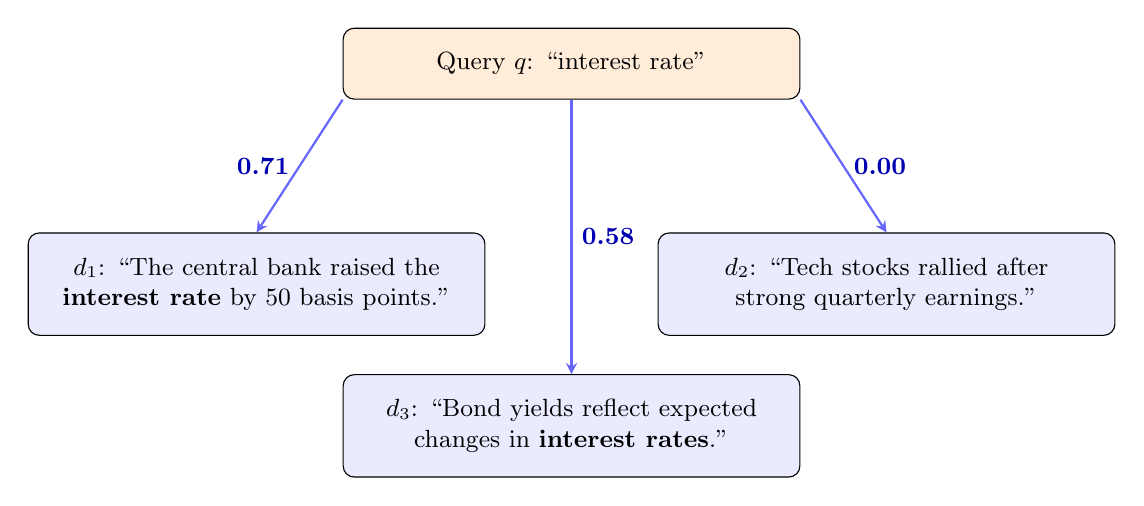
\begin{tikzpicture}[
    doc/.style={draw, rounded corners, fill=blue!8, minimum width=5.8cm,
                minimum height=1.3cm, align=center, font=\small},
    query/.style={draw, rounded corners, fill=orange!15,
                  minimum width=5.8cm, minimum height=0.9cm,
                  align=center, font=\small},
    score/.style={font=\small\bfseries, text=blue!70!black},
    >=stealth
  ]
  % query
  \node[query] (Q) at (0, 3.6)
    {Query $q$: ``interest rate''};
 
  % documents
  \node[doc] (D1) at (-4, 0.8)
    {$d_1$: ``The central bank raised the\\
     \textbf{interest rate} by 50 basis points.''};
  \node[doc] (D2) at (4, 0.8)
    {$d_2$: ``Tech stocks rallied after\\
     strong quarterly earnings.''};
  \node[doc] (D3) at (0, -1.0)
    {$d_3$: ``Bond yields reflect expected\\
     changes in \textbf{interest rates}.''};
 
  % arrows + scores
  \draw[->, thick, blue!60] (Q.south west) -- (D1.north)
    node[midway, left, score] {0.71};
  \draw[->, thick, blue!60] (Q.south east) -- (D2.north)
    node[midway, right, score] {0.00};
  \draw[->, thick, blue!60] (Q.south) -- (D3.north)
    node[midway, right, score] {0.58};
\end{tikzpicture}
\end{center}
 
\smallskip
Documents $d_1$ and $d_3$ score high because they share query terms;
$d_2$ scores zero because it shares none.
The ranking is $d_1 \succ d_3 \succ d_2$.
 
\end{frame}
%
%..................................................................
%
\begin{frame}{The Limits of TF--IDF for Retrieval}

The retrieval mechanism we just described works,
but in practice it produces \textbf{puzzling rankings}.

\bigskip

\begin{tcolorbox}[colback=red!5!white, colframe=red!70!black,
  title=\textbf{Observation 1 --- Term repetition dominates the score}]
If a document repeats a query term many times
(e.g.\ ``inflation'' appears 20 times),
TF--IDF assigns it a much higher weight on that dimension
than a document where the term appears only a few times ---
even when both documents are clearly \emph{about} inflation.
Repeating a word is not the same as being more relevant.
\end{tcolorbox}
\end{frame}
%
%..................................................................
%
\begin{frame}{The Limits of TF--IDF for Retrieval}

\begin{tcolorbox}[colback=red!5!white, colframe=red!70!black,
  title=\textbf{Observation 2 --- Document length skews results}]
Longer documents naturally contain more tokens,
and therefore accumulate higher raw TF counts.
But a 50-page report that mentions ``inflation'' 100 times
is not necessarily more relevant than a concise 1-page analysis
that mentions it 5 times with greater focus.
\end{tcolorbox}

\medskip

Both observations suggest that \textbf{raw term frequency}
is too crude a signal for ranking.
But wait --- didn't we introduce cosine similarity
precisely to neutralize magnitude effects?

\end{frame}
%
%..................................................................
%
\begin{frame}{Wait --- Doesn't Cosine Similarity Already Handle This?}

After seeing these observations, a natural objection arises:

\vspace{0.3cm}
\textbf{Question :  ``We showed that cosine similarity ignores vector magnitude. So shouldn't the normalization cancel out the effect of large TF counts and long documents?''}

\vspace{0.3cm}
The answer involves a crucial distinction:

\begin{columns}[T]
\begin{column}{0.48\textwidth}
\begin{tcolorbox}[colback=green!5!white, colframe=green!60!black,
  title=\textbf{What cosine fixes}]
The \textbf{overall length} of the vector.\\[4pt]
A 100-page document and a 1-page abstract
with the \emph{same term proportions}
will have $\cos\theta = 1$
(identical direction, different magnitude).
\end{tcolorbox}
\end{column}

\begin{column}{0.48\textwidth}
\begin{tcolorbox}[colback=red!5!white, colframe=red!70!black,
  title=\textbf{What cosine does NOT fix}]
The \textbf{direction} of the vector.\\[4pt]
If raw TF inflates one component
disproportionately, the vector \emph{tilts}
toward that dimension.
Cosine faithfully measures this tilted direction
--- it does not correct it.
\end{tcolorbox}
\end{column}
\end{columns}
\end{frame}
%
%..................................................................
%
\begin{frame}{Wait --- Doesn't Cosine Similarity Already Handle This?}

\begin{tcolorbox}[colback=gray!8, colframe=gray!60]
\textbf{Bottom line:} The problems we are about to describe
are problems of the \textbf{TF--IDF weighting scheme} itself,
not of the similarity metric.  They distort the \emph{direction}
of document vectors, and cosine similarity
\emph{preserves} that distortion rather than correcting it.
\end{tcolorbox}

\end{frame}
%
%..................................................................
%
\begin{frame}{Problem 1: Unbounded TF Distorts Vector Direction}
\small
\textbf{Setup.} Vocabulary $V = \{\text{inflation},\, \text{tax},\,
\text{growth}\}$, and suppose $\text{IDF} = 1$ for all terms.

\medskip

\begin{center}
\renewcommand{\arraystretch}{1.2}
\begin{tabular}{l c c c c}
\hline
& inflation & tax & growth & cosine with $q$ \\
\hline
Query $q$  & 1  & 0  & 0 & ---  \\
Doc $A$ (TF=20) & 20 & 5  & 5 & \textbf{0.943} \\
Doc $B$ (TF=10) & 10 & 5  & 5 & \textbf{0.816} \\
\hline
\end{tabular}
\end{center}

\medskip
Doc $A$ mentions ``inflation'' twice as often as $B$,
but both discuss tax and growth equally.
Raw TF \emph{tilts} $A$'s vector more sharply toward the
``inflation'' axis, so cosine gives $A$ a \textbf{16\% higher score}.

\bigskip

\begin{tcolorbox}[colback=red!5!white, colframe=red!70!black,
  title=\textbf{The saturation problem}]
Is document $A$ really more \emph{relevant} than $B$
just because it repeats ``inflation'' more often?
In practice, relevance \textbf{saturates}: once a document
clearly discusses inflation, additional mentions add
\textbf{diminishing informational value}.
Raw TF does not model this saturation ---
it lets the score keep rising with every repetition.
\end{tcolorbox}

\end{frame}
%
%..................................................................
%
\begin{frame}{Problem 2: Document Length Distorts Term Proportions}
\small
Cosine similarity normalizes by vector \emph{norm},
but document length introduces a subtler distortion.

\medskip

\begin{tcolorbox}[colback=red!5!white, colframe=red!70!black,
  title=\textbf{The vocabulary-breadth effect}]
A \textbf{long} document (e.g.\ a 50-page annual report)
covers many topics.  Its TF--IDF vector has \textbf{many non-zero
components} spread across hundreds of terms.\\[4pt]
A \textbf{short} document (e.g.\ a 1-paragraph news flash)
is tightly focused.  Its vector has
\textbf{few non-zero components},
concentrated on the topic at hand.
\end{tcolorbox}

\medskip
\textbf{Effect on cosine similarity with a short query:}

\begin{itemize}
\item The short document's weight is \emph{concentrated}
      on the query terms $\Rightarrow$ high cosine.
\item The long document's weight is \emph{spread}
      across many dimensions $\Rightarrow$ the query-term components
      contribute a smaller share of the norm
      $\Rightarrow$ lower cosine, even if the document discusses
      the topic extensively.
\end{itemize}
\end{frame}
%
%..................................................................
%
\begin{frame}{Problem 2: Document Length Distorts Term Proportions}
\begin{tcolorbox}[colback=gray!8, colframe=gray!60]
\textbf{Paradox:} cosine similarity can \emph{penalize} long,
comprehensive documents in favor of short ones ---
the opposite of the raw-TF bias, but equally undesirable.
A good retrieval function should account for document length
in a \emph{controlled, tunable} way.
\end{tcolorbox}

\end{frame}
%
%..................................................................
%
\begin{frame}{From These Observations to BM25}

\begin{center}
\renewcommand{\arraystretch}{1.4}
\begin{tabular}{l l l}
\hline
\textbf{Problem} & \textbf{Root cause} & \textbf{BM25 solution} \\
\hline
\\
TF saturation & Raw TF grows without bound &
  Saturating function $\dfrac{\text{tf}\cdot(k_1+1)}{\text{tf}+k_1}$ \\[8pt]
Length bias & No explicit length control &
  Normalization factor $1 - b + b\,\dfrac{|d|}{\text{avgdl}}$ \\[8pt]
\hline
\end{tabular}
\end{center}

\begin{tcolorbox}[colback=blue!5!white, colframe=blue!75!black,
  title=\textbf{Historical context}]
These observations motivated \textbf{BM25} (\emph{Best Match~25}),
developed in the 1990s.  It remains the standard sparse-retrieval baseline in 2025. BM25 does \emph{not} use cosine similarity at all ---
it defines its own scoring function that incorporates
saturation and length normalization directly into the formula.
\end{tcolorbox}

\end{frame}
%
%..................................................................
%
\begin{frame}{BM25: Saturated Term Frequency and Length Normalization}
For a query $Q = \{q_1,\dots,q_n\}$ and document $d$:
\[
\mathrm{BM25}(d,Q)\;=\;\sum_{i=1}^{n}
\mathrm{IDF}(q_i)\cdot
\frac{\mathrm{tf}(q_i,d)\cdot(k_1+1)}
     {\displaystyle\mathrm{tf}(q_i,d)+k_1\!\left(1-b+b\,\frac{|d|}{\mathrm{avgdl}}\right)}
\]
 
\vspace{0.12cm}
\begin{columns}[T]
\begin{column}{0.50\textwidth}
\begin{block}{Key parameters}
\begin{itemize}
    \item $k_1\in[1.2,\,2.0]$: \textbf{TF saturation.}\\
    As $\mathrm{tf}\to\infty$, the fraction approaches~$k_1+1$.
    \item $b\approx 0.75$: \textbf{length normalization.}
    \item $|d|$: document length; $\;\mathrm{avgdl}$: corpus average.
\end{itemize}
\end{block}
\end{column}
\begin{column}{0.46\textwidth}
\begin{block}{Special cases}
\begin{itemize}
    \item $b=0$: no length normalization.
    \item $k_1=0$: degenerates to pure IDF.
\end{itemize}
Standard defaults ($k_1\!=\!1.2$, $b\!=\!0.75$) work well across domains without tuning.
\end{block}
\end{column}
\end{columns}
\end{frame}
%
%..................................................................
%
\begin{frame}{BM25: Fixing Both Problems in One Formula}


\medskip

\begin{center}
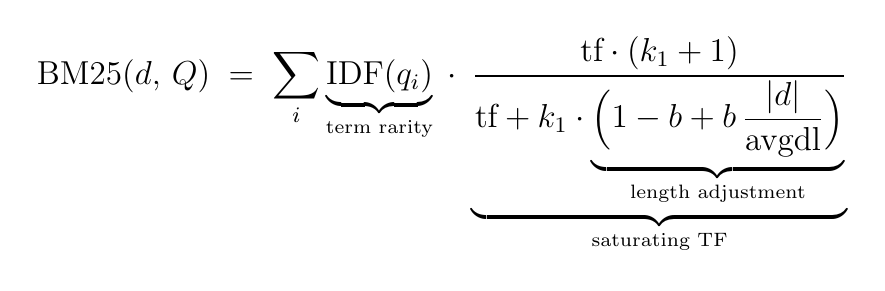
\begin{tikzpicture}[
    brace/.style={decorate, decoration={brace, amplitude=5pt, mirror}},
    ann/.style={font=\scriptsize, align=center},
  ]
  % The formula
  \node[font=\large] (formula) at (0,0) {%
    $\displaystyle
    \text{BM25}(d,\,Q)
    \;=\;
    \sum_{i}
    \underbrace{
      \text{IDF}(q_i)
    }_{\text{\scriptsize term rarity}}
    \;\cdot\;
    \underbrace{
      \frac{\text{tf} \cdot (k_1+1)}
           {\text{tf} + k_1 \cdot
            \underbrace{
              \Bigl(1 - b + b\,\frac{|d|}{\text{avgdl}}\Bigr)
            }_{\text{\scriptsize length adjustment}}
           }
    }_{\text{\scriptsize saturating TF}}
    $};
\end{tikzpicture}
\end{center}
\end{frame}
%
%..................................................................
%
\begin{frame}{BM25: Fixing Both Problems in One Formula}

\begin{columns}[T]
\begin{column}{0.38\textwidth}
\textbf{Reading the formula:}
\begin{itemize}
\item[\color{green!60!black}\textbullet]
  \textbf{IDF}: same role as in TF--IDF ---
  rare terms count more.
\item[\color{blue!70}\textbullet]
  \textbf{Saturating TF}: as tf grows,
  the fraction approaches a ceiling
  ($k_1\!+\!1$) instead of growing forever.
\item[\color{red!70!black}\textbullet]
  \textbf{Length adjustment}: if $|d|$ is longer
  than the corpus average, the denominator
  grows, \emph{dampening} the score.
\end{itemize}
\end{column}

\begin{column}{0.58\textwidth}
\begin{center}
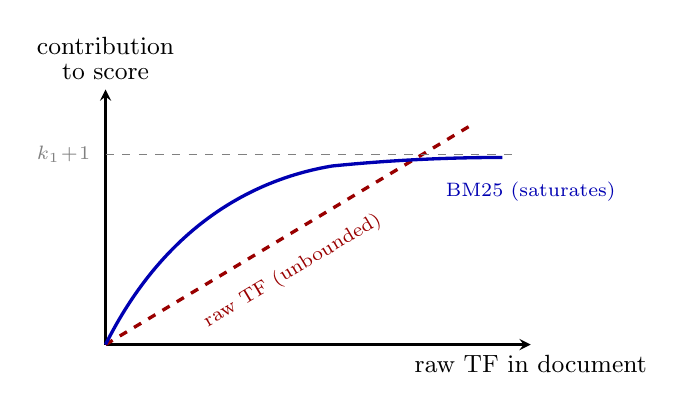
\begin{tikzpicture}[scale=0.72, >=stealth]
  % axes
  \draw[->, thick] (0,0) -- (7.5,0)
    node[below, font=\small] {raw TF in document};
  \draw[->, thick] (0,0) -- (0,4.5)
    node[above, font=\small, align=center] {contribution\\[-2pt]to score};

  % Raw TF: straight line (the problem)
  \draw[red!60!black, very thick, dashed] (0,0) -- (6.5, 3.9);
  \node[font=\scriptsize, red!60!black, rotate=31] at (3.3, 1.3)
    {raw TF (unbounded)};

  % BM25 saturating curve: tf*(k1+1)/(tf+k1), k1=1.5
  % ceiling = k1+1 = 2.5, scaled to ~3.3 on plot
  \draw[blue!70!black, very thick]
    (0, 0)
    .. controls (1.0, 2.0) and (2.5, 2.9) ..
    (4.0, 3.15)
    .. controls (5.0, 3.25) and (6.0, 3.3) ..
    (7.0, 3.3);
  \node[font=\scriptsize, blue!70!black] at (7.5, 2.7)
    {BM25 (saturates)};

  % ceiling line
  \draw[gray, thin, dashed] (0, 3.35) -- (7.2, 3.35);
  \node[font=\scriptsize, gray] at (-0.1, 3.35) [left] {$k_1\!+\!1$};

  % annotation
  %\node[font=\scriptsize, align=center, text=blue!60!black]
  %  at (5.5, 4.3)
  %  {after a few occurrences,\\additional mentions\\barely change the score};
\end{tikzpicture}
\end{center}
\end{column}
\end{columns}

\end{frame}
%
%..................................................................
%
\begin{frame}{BM25 in the Modern Retrieval Pipeline}
\vspace{0.5cm}
\begin{block}{Why BM25 survives in 2025}
\begin{itemize}
    \item No training; fast inference.
    \item Strong on exact-match and rare terms.
    \item Reproducible, well-understood baseline.
    \item Runs on standard inverted indexes.
\end{itemize}
\end{block}
 
\end{frame}
%
%..................................................................
%
\begin{frame}{ }
\begin{center}
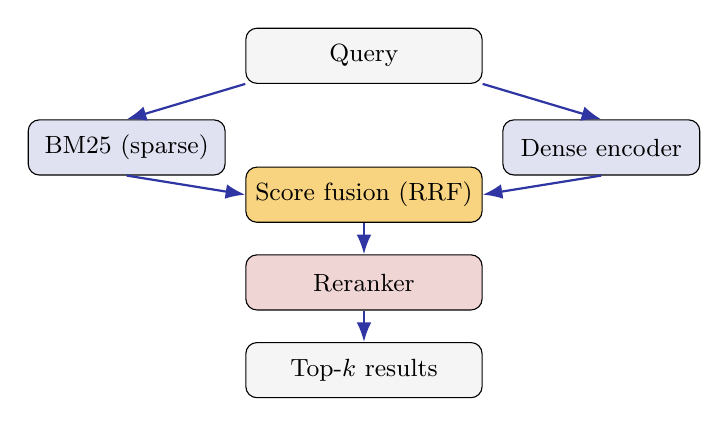
\begin{tikzpicture}[node distance=0.42cm and 0.1cm, every node/.style={font=\small}]
\node[draw, rounded corners, fill=SoftGray,
      minimum width=3.0cm, minimum height=0.7cm] (q) {Query};
\node[draw, rounded corners, fill=CourseBlue!15,
      below left=0.45cm and 0.25cm of q,
      minimum width=2.5cm, minimum height=0.7cm] (bm) {BM25 (sparse)};
\node[draw, rounded corners, fill=CourseBlue!15,
      below right=0.45cm and 0.25cm of q,
      minimum width=2.5cm, minimum height=0.7cm] (de) {Dense encoder};
\node[draw, rounded corners, fill=Accent!50,
      below=1.05cm of q,
      minimum width=3.0cm, minimum height=0.7cm] (fuse) {Score fusion (RRF)};
\node[draw, rounded corners, fill=DeepRed!20,
      below=0.40cm of fuse,
      minimum width=3.0cm, minimum height=0.7cm] (rr) {Reranker};
\node[draw, rounded corners, fill=SoftGray,
      below=0.40cm of rr,
      minimum width=3.0cm, minimum height=0.7cm] (out) {Top-$k$ results};
\draw[-{Latex[length=2.5mm]}, thick, CourseBlue] (q.south west) -- (bm.north);
\draw[-{Latex[length=2.5mm]}, thick, CourseBlue] (q.south east) -- (de.north);
\draw[-{Latex[length=2.5mm]}, thick, CourseBlue] (bm.south) -- (fuse.west);
\draw[-{Latex[length=2.5mm]}, thick, CourseBlue] (de.south)  -- (fuse.east);
\draw[-{Latex[length=2.5mm]}, thick, CourseBlue] (fuse) -- (rr);
\draw[-{Latex[length=2.5mm]}, thick, CourseBlue] (rr)   -- (out);
\end{tikzpicture}
\end{center}

\begin{alertblock}{Forward reference -- Lesson 4}
RAG pipelines run BM25 in parallel with a dense encoder. Outputs are fused via RRF
and reranked before being passed to the LLM.
\end{alertblock}
\end{frame}
%
%..................................................................
%
\begin{frame}{Sparse Vectors and High Dimensionality}
Bag-of-words and TF--IDF vectors are usually:
\begin{itemize}
    \item \textbf{high-dimensional}: vocabulary size can be tens of thousands or more;
    \item \textbf{sparse}: each document contains only a small subset of the vocabulary;
    \item \textbf{interpretable}: each dimension corresponds to a known word.
\end{itemize}

\vspace{0.15cm}
\begin{block}{Strength}
Sparse vectors are simple, transparent, and often surprisingly effective.
\end{block}

\vspace{0.1cm}
\begin{alertblock}{Weakness}
They do not directly encode semantic proximity between different words such as \texttt{car} and \texttt{automobile}.
\end{alertblock}
\end{frame}
%
%..................................................................
%
\begin{frame}{Practical Python Implementation}
\centering
\vspace{1cm}

{\usebeamercolor[fg]{title}\bfseries\LARGE Practical Python Session}

\vspace{0.5cm}

{\large Jupyter Lab}

\vspace{1cm}

\begin{beamercolorbox}[rounded=true, shadow=true, sep=1em, center]{block body}
\begin{minipage}{0.8\textwidth}
\centering
In the next part of the lecture, we will translate the main ideas into code and build a complete workflow in Python.
\end{minipage}
\end{beamercolorbox}

\vspace{0.8cm}

{\normalsize
\textbf{Focus of the lab:} SEC filings, text preprocessing, TF--IDF, and document similarity
}

\vfill

\small 
notebook\_01.ipynb

\end{frame}%__________________________________________________________________________
%
\section{From Sparse Vectors to Word Embeddings}
%__________________________________________________________________________
%
\begin{frame}{Why a New Representation Was Needed}
Two sentences may be semantically close while sharing very few words.

\vspace{0.15cm}
For example:
\begin{align*}
 s_1 &: \texttt{The company announced a merger.}\\
 s_2 &: \texttt{The firm disclosed an acquisition deal.}
\end{align*}

A sparse lexical model may understate their similarity because words such as
\texttt{company}/\texttt{firm} and \texttt{merger}/\texttt{acquisition} occupy different coordinates.

\vspace{0.15cm}
\begin{block}{Goal}
We want a representation where semantically similar words and documents can be geometrically close.
\end{block}
\end{frame}
%
%..................................................................
%
\begin{frame}{What Is a Word Embedding?}
A \textbf{word embedding} maps each word to a dense vector in a low-dimensional continuous space:
\[
 w \longmapsto \vect{e}(w) \in \R^k,
\]
where $k$ is typically much smaller than the vocabulary size.

\vspace{0.15cm}
\begin{block}{Key idea}
Meaning is represented not by an isolated symbol but by the position of a word inside a geometric space learned from data.
\end{block}

\vspace{0.1cm}
Nearby words in that space tend to share similar distributional behavior.
\end{frame}
%
%..................................................................
%
\begin{frame}{The Distributional Hypothesis}
A foundational intuition behind embeddings is the \textbf{distributional hypothesis}:
\begin{center}
\emph{Words that occur in similar contexts tend to have similar meanings.}
\end{center}

\vspace{0.15cm}
\begin{itemize}
    \item If \texttt{bank}, \texttt{lender}, and \texttt{institution} often appear near similar words, their vectors should become similar.
    \item If \texttt{river} and \texttt{shore} appear in another type of local environment, they should form another semantic neighborhood.
\end{itemize}
\end{frame}
%
%..................................................................
%
\begin{frame}{The Company Words Keep}


Consider a small financial corpus:

\begin{tcolorbox}[colback=gray!6, colframe=gray!50,
  fontupper=\small]
\begin{enumerate}
\item The \textbf{bank} approved a new \textbf{loan} for the client.
\item The \textbf{lender} granted a large \textbf{loan} to the firm.
\item The \textbf{bank} increased its \textbf{interest} on deposits.
\item The \textbf{lender} raised the \textbf{interest} rate on mortgages.
\item The \textbf{river} flows under the old stone \textbf{bridge}.
\item The \textbf{river} flooded the \textbf{bridge} after heavy rain.
\end{enumerate}
\end{tcolorbox}

\vspace{0.3cm}
Look at the \textbf{neighbors} of each word.
What words tend to appear near \emph{bank}?
And near \emph{lender}?  And near \emph{river}?

\end{frame}
%
%..................................................................
%
\begin{frame}{Observing the Context Windows}

If we look at which words appear within a window of $\pm 2$ positions
around each target word, we find:

\begin{columns}[T]
\begin{column}{0.32\textwidth}
\begin{tcolorbox}[colback=blue!5!white, colframe=blue!75!black,
  title=\textbf{bank}]
{\small
approved, loan,\\
new, client,\\
increased, interest,\\
its, deposits}
\end{tcolorbox}
\end{column}

\begin{column}{0.32\textwidth}
\begin{tcolorbox}[colback=blue!5!white, colframe=blue!75!black,
  title=\textbf{lender}]
{\small
granted, loan,\\
large, firm,\\
raised, interest,\\
rate, mortgages}
\end{tcolorbox}
\end{column}

\begin{column}{0.32\textwidth}
\begin{tcolorbox}[colback=red!5!white, colframe=red!70!black,
  title=\textbf{river}]
{\small
flows, bridge,\\
under, old,\\
flooded, bridge,\\
after, heavy}
\end{tcolorbox}
\end{column}
\end{columns}

\begin{tcolorbox}[colback=green!5!white, colframe=green!60!black,
  title=\textbf{Key observation}]
\textbf{bank} and \textbf{lender} share context words
(\emph{loan}, \emph{interest}) --- their neighborhoods overlap.\\[4pt]
\textbf{river} shares \emph{none} of these contexts.
It lives in a completely different linguistic environment.
\end{tcolorbox}

\end{frame}
%
%..................................................................
%
\begin{frame}{From Contexts to a Co-occurrence Table}

We can formalize this intuition.
Count how many times each word appears \emph{near}
each other word across the whole corpus:

\begin{center}
\renewcommand{\arraystretch}{1.25}
\begin{tabular}{l | c c c c c c}
             & loan & interest & bridge & approved & granted & flooded \\
\hline
\textbf{bank}   & \textcolor{blue!70}{\textbf{2}} & \textcolor{blue!70}{\textbf{1}} & 0 & \textcolor{blue!50}{\textbf{1}} & 0 & 0 \\
\textbf{lender} & \textcolor{blue!70}{\textbf{2}} & \textcolor{blue!70}{\textbf{1}} & 0 & 0 & \textcolor{blue!50}{\textbf{1}} & 0 \\
\textbf{river}  & 0 & 0 & \textcolor{red!70}{\textbf{2}} & 0 & 0 & \textcolor{red!70}{\textbf{1}} \\
\end{tabular}
\end{center}
\end{frame}
%
%..................................................................
%
\begin{frame}{From Contexts to a Co-occurrence Table}

\begin{tcolorbox}[colback=green!5!white, colframe=green!60!black,
  title=\textbf{Each row is already a vector representation!}]
The row for \emph{bank} $= (2,\,1,\,0,\,1,\,0,\,0)$\\
The row for \emph{lender} $= (2,\,1,\,0,\,0,\,1,\,0)$\\
The row for \emph{river} $= (0,\,0,\,2,\,0,\,0,\,1)$\\[6pt]
The rows for \textbf{bank} and \textbf{lender}
point in a \emph{similar direction}.
The row for \textbf{river} points \emph{elsewhere}.\\[4pt]
\textbf{Semantic similarity has become geometric proximity}.
\end{tcolorbox}

\end{frame}
%
%..................................................................
%
\begin{frame}{The Semantic Map Analogy}


\begin{center}
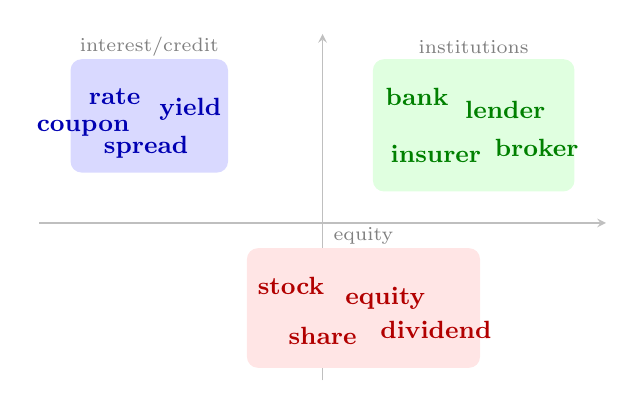
\begin{tikzpicture}[scale=0.8, >=stealth]
  % axes
  \draw[->, gray!50] (-4.5,0) -- (4.5,0);
  \draw[->, gray!50] (0,-2.5) -- (0,3.0);

  % Cluster 1: rates/yields
  \fill[blue!15, rounded corners] (-4.0, 0.8) rectangle (-1.5, 2.6);
  \node[font=\scriptsize, gray] at (-2.75, 2.8) {interest/credit};
  \node[font=\small, blue!70!black] at (-3.3, 2.0) {\textbf{rate}};
  \node[font=\small, blue!70!black] at (-2.1, 1.8) {\textbf{yield}};
  \node[font=\small, blue!70!black] at (-2.8, 1.2) {\textbf{spread}};
  \node[font=\small, blue!70!black] at (-3.8, 1.5) {\textbf{coupon}};

  % Cluster 2: institutions
  \fill[green!12, rounded corners] (0.8, 0.5) rectangle (4.0, 2.6);
  \node[font=\scriptsize, gray] at (2.4, 2.8) {institutions};
  \node[font=\small, green!50!black] at (1.5, 2.0) {\textbf{bank}};
  \node[font=\small, green!50!black] at (2.9, 1.8) {\textbf{lender}};
  \node[font=\small, green!50!black] at (1.8, 1.1) {\textbf{insurer}};
  \node[font=\small, green!50!black] at (3.4, 1.2) {\textbf{broker}};

  % Cluster 3: equity
  \fill[red!10, rounded corners] (-1.2, -2.3) rectangle (2.5, -0.4);
  \node[font=\scriptsize, gray] at (0.65, -0.2) {equity};
  \node[font=\small, red!70!black] at (-0.5, -1.0) {\textbf{stock}};
  \node[font=\small, red!70!black] at (1.0, -1.2) {\textbf{equity}};
  \node[font=\small, red!70!black] at (0.0, -1.8) {\textbf{share}};
  \node[font=\small, red!70!black] at (1.8, -1.7) {\textbf{dividend}};
\end{tikzpicture}
\end{center}

\end{frame}
%
%..................................................................
%
\begin{frame}{So What Do Word2Vec and GloVe Actually Do?}
\footnotesize
The co-occurrence table already captures semantic proximity.
But it has a practical problem:

\begin{tcolorbox}[colback=red!5!white, colframe=red!70!black,
  title=\textbf{The curse of dimensions}]
In a real corpus, the vocabulary may contain
$|V| = 50\,000$ words.\\[4pt]
Each row of the co-occurrence table is a vector in
$\mathbb{R}^{50\,000}$ --- \textbf{extremely sparse}
and expensive to store and compare.
\end{tcolorbox}

\begin{tcolorbox}[colback=green!5!white, colframe=green!60!black,
  title=\textbf{The key idea behind embedding models}]
\textbf{Compress} the co-occurrence information into a much
\textbf{smaller, dense} vector --- typically
$k = 100$--$300$ dimensions.\\[6pt]
\renewcommand{\arraystretch}{1.4}
\begin{tabular}{r c l}
Co-occurrence row & $\longrightarrow$ & Dense embedding \\
$\mathbf{x} \in \mathbb{R}^{50\,000}$ (sparse)
  & & $\mathbf{e} \in \mathbb{R}^{300}$ (dense) \\
\end{tabular}\\[6pt]
The compression preserves the essential structure:
words that were close in the big sparse space
\textbf{remain close} in the small dense space.
\end{tcolorbox}

\bigskip

\begin{tcolorbox}[colback=gray!8, colframe=gray!60]
\textbf{How} this compression is learned
--- through prediction tasks (Word2Vec)
or matrix factorization (GloVe) ---
requires neural-network foundations
that we will develop in \textbf{Lesson~2}.\\[2pt]
For now, the \textbf{what} and the \textbf{why} are clear:
\emph{context patterns in, semantic geometry out.}
\end{tcolorbox}

\end{frame}
%
%..................................................................
%
\begin{frame}{Dense vs Sparse Representations}
\begin{columns}[T]
\begin{column}{0.48\textwidth}
\begin{block}{Sparse lexical vectors}
\begin{itemize}
    \item dimension tied to vocabulary size
    \item mostly zeros
    \item highly interpretable
    \item weak semantic generalization
\end{itemize}
\end{block}
\end{column}
\begin{column}{0.48\textwidth}
\begin{block}{Dense embeddings}
\begin{itemize}
    \item low-dimensional continuous space
    \item almost no zeros
    \item less directly interpretable
    \item stronger semantic generalization
\end{itemize}
\end{block}
\end{column}
\end{columns}

\vspace{0.12cm}
\begin{alertblock}{Trade-off}
The field moves from hand-readable coordinates to learned coordinates that are much more useful for generalization.
\end{alertblock}
\end{frame}
%
%..................................................................
%
\begin{frame}{Embedding Geometry}
In an idealized embedding space, semantic regularities appear as geometric relations.

\vspace{0.15cm}
For example, one may observe patterns of the form:
\[
\vect{e}(\texttt{king}) - \vect{e}(\texttt{man}) + \vect{e}(\texttt{woman}) \approx \vect{e}(\texttt{queen}).
\]

\vspace{0.15cm}
\begin{block}{Interpretation}
The exact analogy should never be taken too literally, but it illustrates a central idea: distributed representations can encode regular semantic and syntactic structure.
\end{block}

\end{frame}
%
%..................................................................
%
\begin{frame}{Static Embeddings and the Role of Context}
Static embeddings assign \textbf{one vector per word type}. Therefore:
\[
\vect{e}(\texttt{bank}) = \text{same vector in all occurrences.}
\]

\vspace{0.15cm}
\begin{block}{This is both powerful and limited}
\begin{itemize}
    \item Powerful: the model learns semantic neighborhoods from co-occurrence patterns.
    \item Limited: the same word may have different meanings in different contexts.
\end{itemize}
\end{block}

\vspace{0.1cm}
This limitation will later motivate contextual embeddings and transformers.
\end{frame}
%
%..................................................................
%
\begin{frame}{Word2Vec: General Idea}
Word2Vec learns embeddings by solving a local prediction problem.

\vspace{0.15cm}
Two main variants are used:
\begin{itemize}
    \item \textbf{CBOW} (Continuous Bag of Words): predict the central word from surrounding context.
    \item \textbf{Skip-Gram}: predict surrounding words from the central word.
\end{itemize}

\vspace{0.15cm}
\begin{block}{Why this matters}
The network is not trained to ``understand semantics'' directly. Semantics emerges because predicting context forces the model to organize words according to their usage environments.
\end{block}
\end{frame}
%
%..................................................................
%
\begin{frame}{Word2Vec: CBOW}
Suppose the context window around a target word is:
\[
(\texttt{the},\texttt{central},\underline{\phantom{bank}},\texttt{raised},\texttt{rates})
\]
CBOW uses the surrounding words to predict the missing central token:
\[
(\texttt{the},\texttt{central},\texttt{raised},\texttt{rates}) \longrightarrow \texttt{bank}
\]

\vspace{0.15cm}
\begin{block}{Intuition}
Words with similar neighboring environments will tend to receive similar embeddings.
\end{block}
\end{frame}
%
%..................................................................
%
\begin{frame}{Word2Vec: Skip-Gram}
Skip-Gram reverses the direction:
\[
\texttt{bank} \longrightarrow (\texttt{central},\texttt{raised},\texttt{rates},\dots)
\]

\vspace{0.15cm}
\begin{block}{Why it is interesting}
A word vector becomes useful if it is informative about the kinds of contexts the word tends to generate.
\end{block}

\vspace{0.12cm}
\begin{itemize}
    \item Frequent words produce many training events.
    \item Nearby words in vector space tend to predict similar local environments.
\end{itemize}
\end{frame}
%
%..................................................................
%
\begin{frame}{The Question We Have Not Yet Answered}

We have established \emph{what} a word embedding is:

\[
  w \;\longmapsto\; \mathbf{e}(w) \in \mathbb{R}^k
  \qquad\text{with } k \ll |V|
\]

And we have seen \emph{why} it is useful: words with similar
contexts receive similar vectors.

\vspace{12pt}
\begin{alertblock}{The missing piece}
\textbf{How} does the training procedure actually produce
these vectors?  Where do the numbers come from?

\vspace{4pt}
We will answer this question using only elementary ideas
--- no neural network formalism is required.
The full machinery (backpropagation, loss functions,
optimizers) will be introduced in Lesson~2.
\end{alertblock}

\end{frame}
%
%..................................................................
%
\begin{frame}{Step 1: The Lookup Table}

Imagine a large spreadsheet with one row per word and $k$~columns
of real numbers.  This spreadsheet \emph{is} the embedding.

\vspace{6pt}
\begin{center}
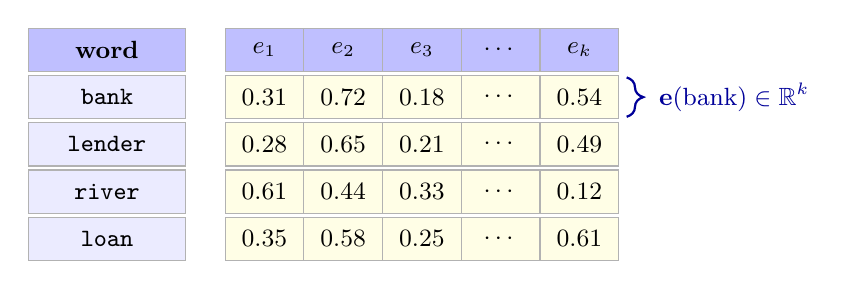
\begin{tikzpicture}[
  cell/.style={minimum width=1.0cm, minimum height=0.55cm,
               draw=gray!60, font=\small},
  wordcell/.style={cell, fill=blue!8, font=\small\ttfamily,
                   minimum width=2.0cm, align=left},
  numcell/.style={cell, fill=yellow!10, font=\small},
  headcell/.style={cell, fill=blue!25, font=\small\bfseries},
]

% Header
\node[headcell, minimum width=2.0cm] (h0) at (0,0) {word};
\node[headcell] (h1) at (2.0,0) {$e_1$};
\node[headcell] (h2) at (3.0,0) {$e_2$};
\node[headcell] (h3) at (4.0,0) {$e_3$};
\node[headcell] (h4) at (5.0,0) {$\cdots$};
\node[headcell] (h5) at (6.0,0) {$e_k$};

% Row: bank
\node[wordcell] at (0,-0.6) {bank};
\node[numcell]  at (2.0,-0.6) {0.31};
\node[numcell]  at (3.0,-0.6) {0.72};
\node[numcell]  at (4.0,-0.6) {0.18};
\node[numcell]  at (5.0,-0.6) {$\cdots$};
\node[numcell]  at (6.0,-0.6) {0.54};

% Row: lender
\node[wordcell] at (0,-1.2) {lender};
\node[numcell]  at (2.0,-1.2) {0.28};
\node[numcell]  at (3.0,-1.2) {0.65};
\node[numcell]  at (4.0,-1.2) {0.21};
\node[numcell]  at (5.0,-1.2) {$\cdots$};
\node[numcell]  at (6.0,-1.2) {0.49};

% Row: river
\node[wordcell] at (0,-1.8) {river};
\node[numcell]  at (2.0,-1.8) {0.61};
\node[numcell]  at (3.0,-1.8) {0.44};
\node[numcell]  at (4.0,-1.8) {0.33};
\node[numcell]  at (5.0,-1.8) {$\cdots$};
\node[numcell]  at (6.0,-1.8) {0.12};

% Row: loan
\node[wordcell] at (0,-2.4) {loan};
\node[numcell]  at (2.0,-2.4) {0.35};
\node[numcell]  at (3.0,-2.4) {0.58};
\node[numcell]  at (4.0,-2.4) {0.25};
\node[numcell]  at (5.0,-2.4) {$\cdots$};
\node[numcell]  at (6.0,-2.4) {0.61};

% Annotation
\draw[decorate, decoration={brace, amplitude=6pt},
      thick, blue!60!black]
  (6.6,-0.35) -- (6.6,-0.85)
  node[midway, right=8pt, font=\small, text=blue!60!black]
  {$\mathbf{e}(\text{bank}) \in \mathbb{R}^k$};

\end{tikzpicture}
\end{center}
\small
\begin{block}{Key point}
Nobody designs these numbers by hand.
At the start of training, every entry is a \textbf{small
random number}.  The training procedure will adjust
them until they encode useful semantic information.
\end{block}

\end{frame}
%
%..................................................................
%
\begin{frame}{Step 2: The Training Game (Skip-Gram)}

Word2Vec learns by playing a simple guessing game, repeated
billions of times over the corpus.

\vspace{8pt}
\begin{center}
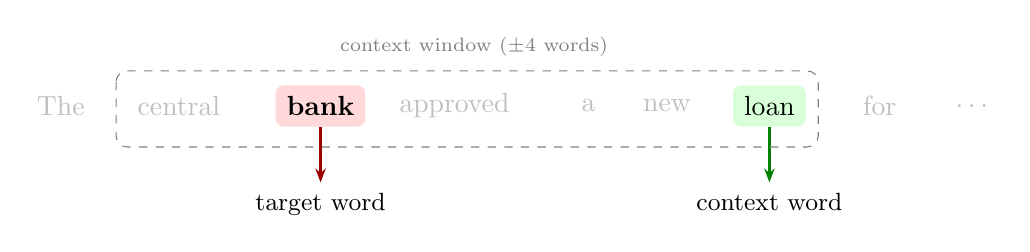
\begin{tikzpicture}[
  word/.style={font=\normalsize, anchor=center},
  target/.style={font=\normalsize\bfseries, 
                 fill=red!15, rounded corners=3pt,
                 inner sep=4pt},
  context/.style={font=\normalsize,
                  fill=green!15, rounded corners=3pt,
                  inner sep=4pt},
  faded/.style={font=\normalsize, text=gray!50},
]

% Sentence
\node[faded]   (w1) at (0,0)   {The};
\node[faded]   (w2) at (1.5,0) {central};
\node[target]  (w3) at (3.3,0) {bank};
\node[faded]   (w4) at (5.0,0) {approved};
\node[faded]   (w5) at (6.7,0) {a};
\node[faded]   (w6) at (7.7,0) {new};
\node[context] (w7) at (9.0,0) {loan};
\node[faded]   (w8) at (10.4,0) {for};
\node[faded]   (w9) at (11.6,0) {\ldots};

% Arrows
\draw[-{Stealth[length=5pt]}, thick, red!60!black]
  (w3.south) -- ++(0,-0.7)
  node[below, font=\small, text=black] {target word};

\draw[-{Stealth[length=5pt]}, thick, green!50!black]
  (w7.south) -- ++(0,-0.7)
  node[below, font=\small, text=black] {context word};

% Window
\draw[dashed, gray, rounded corners=4pt]
  ($(w2.north west)+(-0.15,0.2)$)
  rectangle ($(w7.south east)+(0.15,-0.25)$);
\node[font=\scriptsize, gray, anchor=south]
  at ($(w2.north)!0.5!(w7.north)+(0,0.25)$)
  {context window ($\pm 4$ words)};

\end{tikzpicture}
\end{center}

\vspace{10pt}
\textbf{The game:} given the target word
\colorbox{red!15}{\textbf{bank}}, can the model predict that
\colorbox{green!15}{\textbf{loan}} is one of its neighbors?

\vspace{6pt}
The model's \emph{only} resource for making this prediction
is the lookup table --- the embedding vectors.

\end{frame}
%
%..................................................................
%
\begin{frame}{Step 3: Making a Prediction}

How does the model decide whether \emph{loan} is a plausible
neighbor of \emph{bank}?  With a single operation:
\[
  \text{score}(\text{bank},\, \text{loan})
  \;=\; \mathbf{e}(\text{bank}) \cdot \mathbf{e}(\text{loan})
  \;=\; \sum_{j=1}^{k} e_j(\text{bank})\; e_j(\text{loan})
\]

\begin{itemize}
  \item If the \textbf{dot product is large} $\Rightarrow$
        the model predicts that \emph{loan} is a likely
        neighbor of \emph{bank}.
  \item If the \textbf{dot product is small or negative}
        $\Rightarrow$ the model predicts that the two
        words are unlikely to appear together.
\end{itemize}

\begin{block}{What matters}
The dot product is large when the two vectors point
in a similar direction.  So the model is comparing
\textbf{directions in embedding space} --- exactly
the same geometric idea as cosine similarity.
\end{block}

\end{frame}
%
%..................................................................
%
\begin{frame}{Step 4: Adjusting the Table}

After each prediction, the model checks the answer and makes
a small correction.  The rule is simple in principle:
\small
\begin{columns}[T]
\begin{column}{0.47\textwidth}
\centering
\textbf{Case A: correct pair}\\[2pt]
{\small\emph{bank} and \emph{loan} really do appear together.}

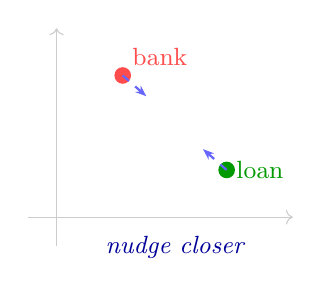
\begin{tikzpicture}[scale=1.2]
  \draw[->, gray!40] (-0.3,0) -- (2.5,0);
  \draw[->, gray!40] (0,-0.3) -- (0,2.0);
  \fill[red!70] (0.7,1.5) circle (2.5pt)
    node[above right, font=\small] {bank};
  \fill[green!60!black] (1.8,0.5) circle (2.5pt)
    node[right, font=\small] {loan};
  \draw[-{Stealth[length=4pt]}, thick, blue!60, dashed]
    (0.7,1.5) -- ++(0.25,-0.22);
  \draw[-{Stealth[length=4pt]}, thick, blue!60, dashed]
    (1.8,0.5) -- ++(-0.25,0.22);
  \node[font=\small\itshape, blue!60!black, anchor=north]
    at (1.25,-0.1) {nudge closer};
\end{tikzpicture}
\end{column}

\begin{column}{0.47\textwidth}
\centering
\textbf{Case B: incorrect pair}\\[2pt]
{\small\emph{bank} and \emph{flood} do not appear together.}

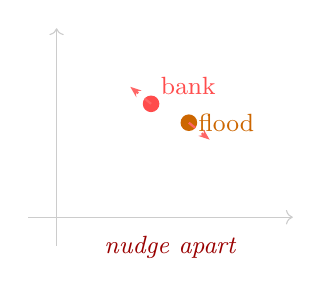
\begin{tikzpicture}[scale=1.2]
  \draw[->, gray!40] (-0.3,0) -- (2.5,0);
  \draw[->, gray!40] (0,-0.3) -- (0,2.0);
  \fill[red!70] (1.0,1.2) circle (2.5pt)
    node[above right, font=\small] {bank};
  \fill[orange!80!black] (1.4,1.0) circle (2.5pt)
    node[right, font=\small] {flood};
  \draw[-{Stealth[length=4pt]}, thick, red!60, dashed]
    (1.0,1.2) -- ++(-0.22,0.18);
  \draw[-{Stealth[length=4pt]}, thick, red!60, dashed]
    (1.4,1.0) -- ++(0.22,-0.18);
  \node[font=\small\itshape, red!60!black, anchor=north]
    at (1.2,-0.1) {nudge apart};
\end{tikzpicture}
\end{column}
\end{columns}

\vspace{4pt}
\begin{block}{That is the entire mechanism}
Pull together vectors of words that co-occur.
Push apart vectors of words that do not.
Repeat billions of times. The final positions
encode distributional similarity.
\end{block}

\end{frame}
%
%..................................................................
%
\begin{frame}{A Toy Example: Before Training}

Suppose our vocabulary has six words and we use $k=2$
dimensions (so we can draw them).

\vspace{4pt}
\begin{columns}[c]
\begin{column}{0.42\textwidth}
\small
\begin{center}
\begin{tabular}{lrr}
\toprule
\textbf{word} & $e_1$ & $e_2$ \\
\midrule
bank     &  0.12 & $-$0.34 \\
lender   & $-$0.51 &  0.27 \\
loan     &  0.43 &  0.08 \\
river    &  0.05 &  0.39 \\
flood    & $-$0.29 & $-$0.18 \\
bridge   &  0.33 & $-$0.41 \\
\bottomrule
\end{tabular}
\end{center}
\vspace{4pt}
{\small All entries are \textbf{small random numbers}.
No structure at all.}
\end{column}
\begin{column}{0.55\textwidth}
\centering
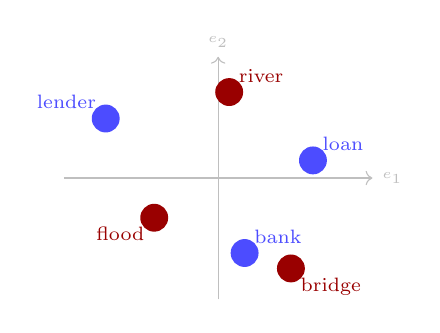
\begin{tikzpicture}[scale=2.8]
  \draw[->, gray!50] (-0.7,0) -- (0.7,0)
    node[right, font=\tiny] {$e_1$};
  \draw[->, gray!50] (0,-0.55) -- (0,0.55)
    node[above, font=\tiny] {$e_2$};

  % Points - random positions
  \fill[blue!70]         ( 0.12,-0.34) circle (1.8pt)
    node[above right, font=\scriptsize] {bank};
  \fill[blue!70]         (-0.51, 0.27) circle (1.8pt)
    node[above left, font=\scriptsize]  {lender};
  \fill[blue!70]         ( 0.43, 0.08) circle (1.8pt)
    node[above right, font=\scriptsize] {loan};
  \fill[red!60!black]    ( 0.05, 0.39) circle (1.8pt)
    node[above right, font=\scriptsize] {river};
  \fill[red!60!black]    (-0.29,-0.18) circle (1.8pt)
    node[below left, font=\scriptsize]  {flood};
  \fill[red!60!black]    ( 0.33,-0.41) circle (1.8pt)
    node[below right, font=\scriptsize] {bridge};
\end{tikzpicture}

\vspace{2pt}
{\small\itshape Before training: scattered randomly.}
\end{column}
\end{columns}

\end{frame}
%
%..................................................................
%
\begin{frame}{A Toy Example: After Training}

After billions of such adjustments over the entire corpus:

\vspace{4pt}
\begin{columns}[c]
\begin{column}{0.42\textwidth}
\small
\begin{center}
\begin{tabular}{lrr}
\toprule
\textbf{word} & $e_1$ & $e_2$ \\
\midrule
bank     &  0.71 &  0.63 \\
lender   &  0.62 &  0.52 \\
loan     &  0.74 &  0.50 \\
river    & $-$0.52 & $-$0.61 \\
flood    & $-$0.48 & $-$0.45 \\
bridge   & $-$0.60 & $-$0.49 \\
\bottomrule
\end{tabular}
\end{center}
\vspace{4pt}
{\small Rows that were random now show
\textbf{clear clusters}.}
\end{column}
\begin{column}{0.55\textwidth}
\centering
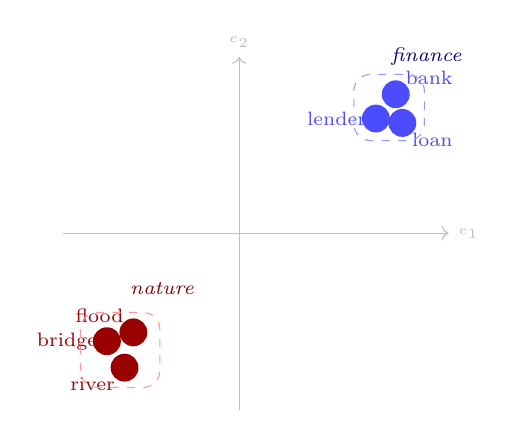
\begin{tikzpicture}[scale=2.8]
  \draw[->, gray!50] (-0.8,0) -- (0.95,0)
    node[right, font=\tiny] {$e_1$};
  \draw[->, gray!50] (0,-0.8) -- (0,0.8)
    node[above, font=\tiny] {$e_2$};

  % Finance cluster
  \fill[blue!70]         ( 0.71, 0.63) circle (1.8pt)
    node[above right, font=\scriptsize] {bank};
  \fill[blue!70]         ( 0.62, 0.52) circle (1.8pt)
    node[left, font=\scriptsize]  {lender};
  \fill[blue!70]         ( 0.74, 0.50) circle (1.8pt)
    node[below right, font=\scriptsize] {loan};

  % Nature cluster
  \fill[red!60!black]    (-0.52,-0.61) circle (1.8pt)
    node[below left, font=\scriptsize] {river};
  \fill[red!60!black]    (-0.48,-0.45) circle (1.8pt)
    node[above left, font=\scriptsize]  {flood};
  \fill[red!60!black]    (-0.60,-0.49) circle (1.8pt)
    node[left, font=\scriptsize] {bridge};

  % Cluster outlines
  \draw[blue!40, dashed, rounded corners=6pt]
    (0.52,0.42) rectangle (0.84,0.72);
  \draw[red!40, dashed, rounded corners=6pt]
    (-0.72,-0.70) rectangle (-0.36,-0.36);

  % Labels
  \node[font=\scriptsize\itshape, blue!50!black]
    at (0.85,0.8) {finance};
  \node[font=\scriptsize\itshape, red!50!black]
    at (-0.35,-0.25) {nature};

\end{tikzpicture}

\vspace{2pt}
{\small\itshape After training: semantic clusters emerge.}
\end{column}
\end{columns}

\end{frame}
%
%..................................................................
%
\begin{frame}{A Toy Example: After Training (more Realistic!}

After billions of such adjustments over the entire corpus:

\vspace{4pt}
\begin{columns}[c]
\begin{column}{0.42\textwidth}
\small
\begin{center}
\begin{tabular}{lrr}
\toprule
\textbf{word} & $e_1$ & $e_2$ \\
\midrule
bank     &  0.71 &  0.63 \\
lender   &  0.62 &  0.52 \\
loan     &  0.74 &  0.50 \\
river    & $-$0.52 & $-$0.61 \\
flood    & $-$0.48 & $-$0.45 \\
bridge   & $-$0.60 & $-$0.49 \\
\bottomrule
\end{tabular}
\end{center}
\vspace{4pt}
{\small Rows that were random now show
\textbf{clear clusters}.}
\end{column}
\begin{column}{0.55\textwidth}
\centering
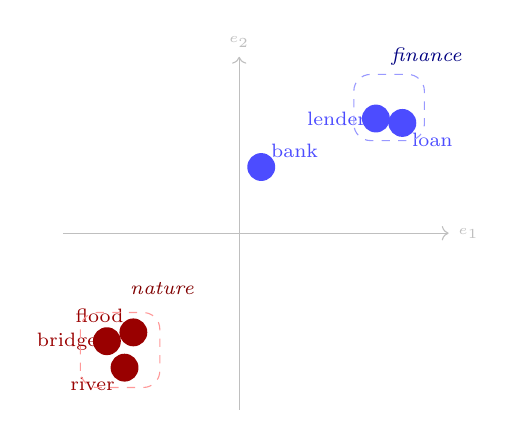
\begin{tikzpicture}[scale=2.8]
  \draw[->, gray!50] (-0.8,0) -- (0.95,0)
    node[right, font=\tiny] {$e_1$};
  \draw[->, gray!50] (0,-0.8) -- (0,0.8)
    node[above, font=\tiny] {$e_2$};

  % Finance cluster
  \fill[blue!70]         ( 0.1, 0.3) circle (1.8pt)
    node[above right, font=\scriptsize] {bank};
  \fill[blue!70]         ( 0.62, 0.52) circle (1.8pt)
    node[left, font=\scriptsize]  {lender};
  \fill[blue!70]         ( 0.74, 0.50) circle (1.8pt)
    node[below right, font=\scriptsize] {loan};

  % Nature cluster
  \fill[red!60!black]    (-0.52,-0.61) circle (1.8pt)
    node[below left, font=\scriptsize] {river};
  \fill[red!60!black]    (-0.48,-0.45) circle (1.8pt)
    node[above left, font=\scriptsize]  {flood};
  \fill[red!60!black]    (-0.60,-0.49) circle (1.8pt)
    node[left, font=\scriptsize] {bridge};

  % Cluster outlines
  \draw[blue!40, dashed, rounded corners=6pt]
    (0.52,0.42) rectangle (0.84,0.72);
  \draw[red!40, dashed, rounded corners=6pt]
    (-0.72,-0.70) rectangle (-0.36,-0.36);

  % Labels
  \node[font=\scriptsize\itshape, blue!50!black]
    at (0.85,0.8) {finance};
  \node[font=\scriptsize\itshape, red!50!black]
    at (-0.35,-0.25) {nature};

\end{tikzpicture}

\vspace{2pt}
{\small\itshape After training: semantic clusters emerge.}
\end{column}
\end{columns}

\end{frame}
%
%..................................................................
%
\begin{frame}{GloVe: Another Route to Dense Representations}
GloVe stands for \textbf{Global Vectors for Word Representation}. It combines two ideas:
\begin{itemize}
    \item local co-occurrence information, as in prediction-based models;
    \item global corpus statistics, summarized by a co-occurrence matrix.
\end{itemize}

\vspace{0.15cm}
\begin{block}{Co-occurrence matrix}
Entry $X_{ij}$ records how often word $w_j$ appears in the context of word $w_i$.
\end{block}
\end{frame}
%
%..................................................................
%
\begin{frame}{Why Co-occurrence Matters}
If two words tend to appear in similar neighborhoods, their co-occurrence profiles should be similar.

\vspace{0.15cm}
\begin{block}{Example}
If \texttt{bank} frequently co-occurs with \texttt{loan}, \texttt{interest}, and \texttt{deposit}, while \texttt{riverbank} co-occurs with \texttt{water}, \texttt{shore}, and \texttt{flood}, then a useful representation should preserve this distinction.
\end{block}

\vspace{0.12cm}
GloVe starts from a large table of word co-occurrences. It then learns dense vectors that preserve the main statistical relationships in that table. In this way, words that appear in similar linguistic environments become close in the embedding space.

\end{frame}
%
%..................................................................
%
\begin{frame}{Sparse to Dense: What We Gain and What We Lose}
\begin{columns}[T]
\begin{column}{0.48\textwidth}
\begin{block}{What we gain}
\begin{itemize}
    \item semantic smoothness
    \item generalization across vocabulary
    \item useful initialization for downstream tasks
    \item better handling of synonymy and analogy
\end{itemize}
\end{block}
\end{column}
\begin{column}{0.48\textwidth}
\begin{block}{What we lose}
\begin{itemize}
    \item easy interpretability of each dimension
    \item direct lexical transparency
    \item a simple one-feature-one-word reading
\end{itemize}
\end{block}
\end{column}
\end{columns}
\end{frame}
%
%..................................................................
%
\begin{frame}{From Word Vectors to Document Vectors}
Word embeddings assign a vector to each \emph{word}. But many downstream tasks ---
retrieval, classification, clustering --- require a vector for an entire \emph{document}.

\vspace{0.15cm}
\begin{block}{The simplest bridge: mean pooling}
Given a document $d = (w_1,\dots,w_L)$ with word embeddings $\vect{e}(w_i)$:
\[
\vect{d}_{\text{mean}} = \frac{1}{L}\sum_{i=1}^{L}\vect{e}(w_i).
\]
\end{block}

\end{frame}
%
%..................................................................
%
\begin{frame}{From Word Vectors to Document Vectors}
Word embeddings assign a vector to each \emph{word}. But many downstream tasks ---
retrieval, classification, clustering --- require a vector for an entire \emph{document}.

\vspace{0.15cm}
\begin{block}{Weighted averaging}
A common refinement weights each word by its TF--IDF score:
\[
\vect{d}_{\text{tfidf}} = \frac{\sum_{i=1}^{L} \mathrm{tfidf}(w_i,d,D)\;\vect{e}(w_i)}
{\sum_{i=1}^{L} \mathrm{tfidf}(w_i,d,D)}.
\]
This down-weights frequent, uninformative words and up-weights distinctive terms ---
combining the strengths of sparse weighting with dense geometry.
\end{block}
\end{frame}
%
%..................................................................
%
\begin{frame}{Document Embeddings: Beyond Simple Averaging}
\small
\begin{columns}[T]
\begin{column}{0.50\textwidth}
\begin{block}{Doc2Vec (Le \& Mikolov, 2014)}
Extends Word2Vec by introducing a learnable \textbf{paragraph vector} that participates
in the prediction task alongside word embeddings. Each document receives its own
trainable vector.
\end{block}

\vspace{0.10cm}
\begin{block}{SIF embeddings (Arora et al., 2017)}
A theoretically motivated scheme:
\begin{enumerate}
    \item compute weighted average using smooth inverse frequency weights;
    \item remove the first principal component (common discourse vector).
\end{enumerate}
Surprisingly competitive with more complex models.
\end{block}
\end{column}
\begin{column}{0.46\textwidth}
\begin{block}{Modern sentence encoders}
Models like Sentence-BERT (2019) and the current generation of embedding models
(\texttt{e5}, \texttt{GTE}, \texttt{nomic-embed}) produce document-level dense vectors
directly from transformer encoders. These are the backbone of modern semantic search.

\vspace{0.10cm}
$\Rightarrow$ \textbf{Lesson~2} will explain the neural foundations;\\
$\Rightarrow$ \textbf{Lesson~4} will show how these vectors drive retrieval and RAG.
\end{block}
\end{column}
\end{columns}

\vspace{0.12cm}
\begin{alertblock}{The key question}
How do we get from a bag of static word vectors to a single vector that captures meaning?
The answer requires understanding \emph{learned} representations --- the subject of the next lesson.
\end{alertblock}
\end{frame}
%
%..................................................................
%
\begin{frame}{The Complementarity of Sparse and Dense}
Now that we have seen both sparse and dense representations, we can appreciate their
\textbf{complementary} failure modes:
\small 
\vspace{0.12cm}
\begin{columns}[T]
\begin{column}{0.48\textwidth}
\begin{block}{Sparse fails at semantics}
\texttt{monetary tightening} does not match a document containing only
\texttt{interest rate hike}, although they are equivalent in meaning.
Sparse methods require lexical overlap.
\end{block}
\end{column}
\begin{column}{0.48\textwidth}
\begin{block}{Dense fails at precision}
An embedding model may rank a document about \texttt{Apple Inc.}\ highly
for a query about \texttt{apple orchards} because their representations
overlap in geometric space.
\end{block}
\end{column}
\end{columns}
 
\vspace{0.18cm}
\begin{block}{Hybrid retrieval}
Combine sparse and dense signals. Each component compensates for the other's blind spot.
This is the architecture underlying most production-grade search and RAG systems in 2025.
Score fusion is typically performed via \textbf{Reciprocal Rank Fusion (RRF)}, which
combines the two ranked lists by position rather than by raw score -- no calibration required.
\end{block}
\end{frame}
%
%..................................................................
%
\begin{frame}{The Importance of Context}
Static embeddings are a major improvement over sparse lexical vectors, but they still assign a single vector to each word type.

\vspace{0.15cm}
\begin{block}{Problem}
The word \texttt{current} in
\begin{itemize}
    \item \texttt{current news}
    \item \texttt{electric current}
\end{itemize}
should not have exactly the same representation in both cases.
\end{block}

\vspace{0.15cm}
This is where the field begins to move toward \textbf{contextual embeddings}, which will be the topic of the next lesson.
\end{frame}
%
%..................................................................
%
\begin{frame}{A Compact Comparison of Representational Stages}
\small
\begin{center}
\begin{tabular}{p{0.22\textwidth}p{0.14\textwidth}p{0.26\textwidth}p{0.26\textwidth}}
\toprule
\textbf{Stage} & \textbf{Unit} & \textbf{Representation} & \textbf{Main limitation} \\
\midrule
BoW / TF--IDF & document & sparse lexical weights & ignores semantics and order \\[3pt]
Word2Vec / GloVe & word type & dense static vector & ignores context; one vector per type \\[3pt]
Doc averaging / Doc2Vec & document & dense static (pooled) & still no context sensitivity \\[3pt]
Contextual models & token in context & context-dependent vector & more complex and less transparent \\
\bottomrule
\end{tabular}
\end{center}

\vspace{0.12cm}
\begin{alertblock}{Forward reference -- byte-level models}
The most recent architectures (ByT5, MegaByte, byte-latent transformers) explore
\textbf{eliminating subword tokenization entirely}, operating directly on raw bytes.
This may reshape how financial text, numbers, and tickers enter language models ---
a theme we revisit in Lesson~3.
\end{alertblock}
\end{frame}
%__________________________________________________________________________
%
\section{Conclusion and Transition}
%__________________________________________________________________________
%
\begin{frame}{What We Have Learned Today}
\begin{itemize}
    \item Text must be transformed into numerical structure before we can learn from it.
    \item Classical NLP begins with corpora, preprocessing, and sparse vector representations.
    \item Bag-of-words, TF--IDF, and BM25 remain important because they make the feature space explicit, interpretable, and surprisingly competitive.
    \item Word embeddings replace sparse lexical coordinates with dense distributed representations; document-level vectors can be derived by pooling or learning.
    \item Sparse and dense methods have complementary failure modes; modern retrieval systems combine both.
    \item Static embeddings improve semantic generalization, but they do not solve context dependence --- the topic of our next lesson.
\end{itemize}
\end{frame}
%
%..................................................................
%
\begin{frame}{Main Takeaways}
\begin{block}{Takeaway 1}
A representation is never neutral: every representation encodes assumptions about what matters in language.
\end{block}

\begin{block}{Takeaway 2}
Sparse lexical models are still useful, but they cannot fully capture semantic proximity or contextual meaning.
\end{block}

\begin{block}{Takeaway 3}
The move from counts to embeddings is not a cosmetic improvement: it is the beginning of a new representational regime in NLP.
\end{block}
\end{frame}
%
%..................................................................
%
\begin{frame}{Looking Ahead to Lesson 2}
In the next lesson, we will deepen the transition that begins today.

\vspace{0.15cm}
We will study:
\begin{itemize}
    \item why neural networks matter for language representations;
    \item how a model can learn features instead of relying on manual feature engineering;
    \item how contextual embeddings emerge from self-attention and transformer architectures.
\end{itemize}

\vspace{0.18cm}
\begin{alertblock}{Bridge to the next step}
Today we learned how to turn text into vectors. Next time we will ask a deeper question: \textbf{how can a model learn the right representation by itself, and how does context change the meaning of a token?}
\end{alertblock}
\end{frame}
%__________________________________________________________________________
%
\section{Appendix}
%__________________________________________________________________________
%
%
%..................................................................
%
\begin{frame}{Appendix 1 --- The Statistical Structure of Language: Zipf's Law}
An empirical regularity that shapes every natural-language corpus:
 
\vspace{0.12cm}
\begin{block}{Zipf's law (G.\ K.\ Zipf, 1949)}
If words are ranked by frequency, the frequency of the $r$-th most common word
satisfies:
\[
\mathrm{freq}(r) \;\propto\; \frac{1}{r^{\,\alpha}}, \qquad \alpha \approx 1.
\]
\end{block}
 
\vspace{0.12cm}
Immediate consequences:
\begin{itemize}
    \item A handful of words (\texttt{the}, \texttt{of}, \texttt{and}, \dots) accounts for
    roughly \textbf{50\,\%} of all tokens in a typical English corpus.
    \item A large fraction of the vocabulary consists of \textbf{hapax legomena}: words
    appearing exactly once.
    \item Raw count vectors are dominated by high-frequency, low-information words.
\end{itemize}
\end{frame}
%
%..................................................................
%
\begin{frame}{Appendix 1 --- Zipf's Law: Why It Matters for Text Representation}
\begin{columns}[T]
\begin{column}{0.50\textwidth}
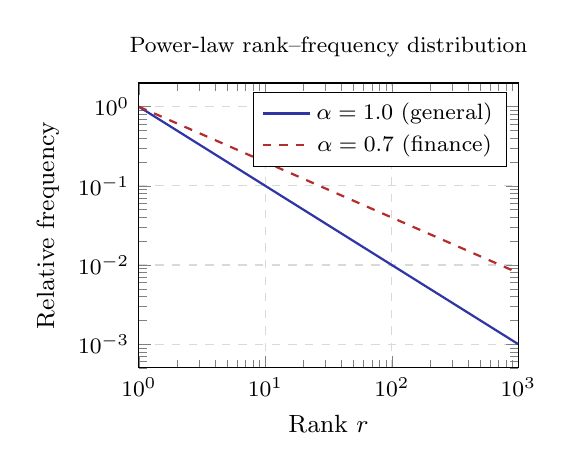
\begin{tikzpicture}
\begin{loglogaxis}[
    width=6.4cm, height=5.2cm,
    xlabel={Rank $r$},
    ylabel={Relative frequency},
    xlabel style={font=\small},
    ylabel style={font=\small},
    tick label style={font=\footnotesize},
    grid=major,
    grid style={dashed,gray!30},
    domain=1:1000, samples=100,
    xmin=1, xmax=1000,
    legend style={font=\footnotesize,
        at={(0.97,0.97)}, anchor=north east},
    title={\footnotesize Power-law rank--frequency distribution},
    title style={font=\footnotesize},
]
\addplot[thick, CourseBlue] {1/x};
\addplot[dashed, DeepRed, thick] {1/x^0.7};
\legend{$\alpha=1.0$ (general), $\alpha=0.7$ (finance)}
\end{loglogaxis}
\end{tikzpicture}
\end{column}
\begin{column}{0.46\textwidth}
\begin{block}{Connection to IDF}
IDF is a statistical correction for Zipf's law. It penalizes the terms that cluster
at the top of the frequency distribution -- ubiquitous but discriminatively empty.
\end{block}
 
\begin{block}{Financial corpora}
Domain terms (\texttt{EBITDA}, \texttt{haircut}, \texttt{collateral call}) are rare
in general language but informationally dense. They receive high IDF weights -- and
hence high TF--IDF scores when prominent in a document.
\end{block}

\end{column}
\end{columns}
\end{frame}
%
%..................................................................
%
\begin{frame}{Appendix 2 --- The Score Fusion Problem}

In a hybrid retrieval pipeline, two (or more) independent systems
each return a \textbf{ranked list} of documents for the same query.

\bigskip

\begin{columns}[T]
\begin{column}{0.45\textwidth}
\begin{tcolorbox}[colback=blue!5!white, colframe=blue!75!black,
  title=\textbf{BM25 (sparse)}]
\renewcommand{\arraystretch}{1.15}
\begin{tabular}{c l r}
Rank & Doc & Score \\
\hline
1 & $d_3$ & 18.7 \\
2 & $d_1$ & 12.4 \\
3 & $d_5$ & 9.1 \\
4 & $d_2$ & 6.3 \\
5 & $d_4$ & 2.8 \\
\end{tabular}
\end{tcolorbox}
\end{column}

\begin{column}{0.45\textwidth}
\begin{tcolorbox}[colback=red!5!white, colframe=red!70!black,
  title=\textbf{Dense encoder}]
\renewcommand{\arraystretch}{1.15}
\begin{tabular}{c l r}
Rank & Doc & Score \\
\hline
1 & $d_1$ & 0.93 \\
2 & $d_3$ & 0.88 \\
3 & $d_7$ & 0.81 \\
4 & $d_5$ & 0.79 \\
5 & $d_6$ & 0.72 \\
\end{tabular}
\end{tcolorbox}
\end{column}
\end{columns}
\end{frame}
%
%..................................................................
%
\begin{frame}{Appendix 2 --- The Score Fusion Problem}

\begin{tcolorbox}[colback=orange!5!white, colframe=orange!70!black,
  title=\textbf{The problem}]
How do we merge these two lists into a \emph{single} ranking?\\[4pt]
We \textbf{cannot} simply average the scores:
BM25 produces unbounded values (18.7, 12.4, \ldots)
while the dense encoder produces cosine similarities in $[0,\,1]$.
The two scales are \textbf{incommensurable}.
\end{tcolorbox}

\end{frame}
%
%..................................................................
%
\begin{frame}{Appendix 2 --- Reciprocal Rank Fusion: The Idea}

\textbf{Key insight:} ignore the raw scores entirely.
Use only the \textbf{position} (rank) of each document in each list.

\bigskip

\begin{tcolorbox}[colback=blue!5!white, colframe=blue!75!black,
  title=\textbf{RRF formula}]
Given $R$ ranked lists, the fused score of document $d$ is:
\[
  \text{RRF}(d)
  \;=\;
  \sum_{r=1}^{R}
  \frac{1}{k \;+\; \text{rank}_r(d)}
\]
where $\text{rank}_r(d)$ is the position of $d$ in the $r$-th list
(1 = top), and $k$ is a smoothing constant (typically $k=60$).
\end{tcolorbox}
\end{frame}
%
%..................................................................
%
\begin{frame}{Appendix 2 --- Reciprocal Rank Fusion: The Idea}

\textbf{Why this works:}
\begin{itemize}
\item A document ranked \textbf{high} in a list receives a
      \textbf{large} reciprocal ($\frac{1}{61} \approx 0.0164$
      for rank 1).
\item A document ranked \textbf{low} receives a
      \textbf{small} reciprocal ($\frac{1}{70} \approx 0.0143$
      for rank 10).
\item A document that does \textbf{not appear} in a list
      is treated as having rank $= \infty$, contributing $\approx 0$.
\item The constant $k=60$ prevents the top-ranked document
      from dominating excessively: the difference between
      rank~1 and rank~2 is $\frac{1}{61} - \frac{1}{62} \approx 0.0003$,
      not a factor of~2.
\end{itemize}

\end{frame}
%
%..................................................................
%
\begin{frame}{Appendix 2 --- RRF: Worked Example ($k=60$)}

Using the two lists from the previous slide:

\bigskip

\begin{center}
\renewcommand{\arraystretch}{1.3}
\begin{tabular}{l c c c c l}
\hline
\textbf{Doc}
  & \textbf{BM25 rank}
  & $\frac{1}{60+\text{rank}}$
  & \textbf{Dense rank}
  & $\frac{1}{60+\text{rank}}$
  & \textbf{RRF score} \\
\hline
$d_1$ & 2 & $\frac{1}{62} = .0161$
      & 1 & $\frac{1}{61} = .0164$
      & $\mathbf{.0325}$ \\[3pt]
$d_3$ & 1 & $\frac{1}{61} = .0164$
      & 2 & $\frac{1}{62} = .0161$
      & $\mathbf{.0325}$ \\[3pt]
$d_5$ & 3 & $\frac{1}{63} = .0159$
      & 4 & $\frac{1}{64} = .0156$
      & $.0315$ \\[3pt]
$d_7$ & --- & $\approx 0$
      & 3 & $\frac{1}{63} = .0159$
      & $.0159$ \\[3pt]
$d_2$ & 4 & $\frac{1}{64} = .0156$
      & --- & $\approx 0$
      & $.0156$ \\[3pt]
$d_6$ & --- & $\approx 0$
      & 5 & $\frac{1}{65} = .0154$
      & $.0154$ \\[3pt]
$d_4$ & 5 & $\frac{1}{65} = .0154$
      & --- & $\approx 0$
      & $.0154$ \\
\hline
\end{tabular}
\end{center}
\end{frame}
%
%..................................................................
%
\begin{frame}{Appendix 2 --- RRF: Worked Example ($k=60$)}
\begin{tcolorbox}[colback=green!5!white, colframe=green!60!black,
  title=\textbf{Fused ranking}]
$d_1 \approx d_3 \;\succ\; d_5 \;\succ\; d_7 \;\succ\; d_2
\;\approx\; d_6 \;\approx\; d_4$\\[4pt]
Documents $d_1$ and $d_3$ tie because they hold symmetric positions.
$d_5$ ranks third because it appears in \textbf{both} lists,
while $d_7$, $d_2$, $d_6$, $d_4$ each appear in only one.
\end{tcolorbox}

\end{frame}
%
%..................................................................
%
\begin{frame}{Appendix 2 --- Why RRF Is the Default Fusion Method}
\footnotesize
\begin{columns}[T]
\begin{column}{0.48\textwidth}
\begin{tcolorbox}[colback=green!5!white, colframe=green!60!black,
  title=\textbf{Advantages}]
\begin{itemize}
\item \textbf{No calibration needed.}
      Works with any combination of rankers
      regardless of their score scales.
\item \textbf{No training data.}
      A single hyperparameter ($k$) with a
      robust default ($k=60$).
\item \textbf{Rewards consensus.}
      Documents ranked highly by \emph{multiple}
      systems float to the top.
\item \textbf{Extensible.}
      Adding a third ranker is trivial ---
      just add another term to the sum.
\end{itemize}
\end{tcolorbox}
\end{column}

\begin{column}{0.48\textwidth}
\begin{tcolorbox}[colback=red!5!white, colframe=red!70!black,
  title=\textbf{Limitations}]
\begin{itemize}
\item \textbf{Ignores score magnitude.}
      A document ranked 1st with score 0.99
      and one ranked 1st with score 0.51
      are treated identically.
\item \textbf{Equal weight to all rankers.}
      If one ranker is much better than the other,
      RRF does not know this.
\item \textbf{Truncation matters.}
      If a ranker returns only top-100 documents,
      anything beyond that cutoff is invisible.
\end{itemize}
\end{tcolorbox}

%\begin{tcolorbox}[colback=gray!8, colframe=gray!60]
%{\small Despite these limitations, RRF is the
%most widely used fusion method in production
%RAG systems as of 2025.}
%\end{tcolorbox}
\end{column}
\end{columns}

\end{frame}
%
%===================================================================================================
%
\end{document}

%
%..................................................................
%
\begin{frame}{SPLADE: Learned Sparse Representations}
\textbf{SPLADE} (SParse Lexical AnD Expansion, 2021--2022) bridges the gap between
interpretability and neural expressiveness.
 
\vspace{0.12cm}
\begin{columns}[T]
\begin{column}{0.52\textwidth}
\begin{block}{Core idea}
A transformer encoder produces a \textbf{sparse vector in vocabulary space}:
\[
\vect{s}(d)\in\R^{|V|},\qquad \|\vect{s}(d)\|_0 \ll |V|.
\]
Non-zero entries correspond to terms deemed relevant -- including terms \textbf{not
literally present} in the input (\emph{query and document expansion}).
\end{block}
\end{column}
\begin{column}{0.44\textwidth}
\begin{block}{Properties}
\begin{itemize}
    \item Each dimension is a vocabulary term $\Rightarrow$ \textbf{interpretable}.
    \item Sparse $\Rightarrow$ standard inverted-index compatible.
    \item Learned $\Rightarrow$ handles synonyms and paraphrases.
    \item Performance approaches dense models with sparse efficiency.
\end{itemize}
\end{block}
\end{column}
\end{columns}
\end{frame}
%
%..................................................................
%
\begin{frame}{A Positioning Map of Retrieval Representations}
\begin{columns}[T]
\begin{column}{0.55\textwidth}
\begin{center}
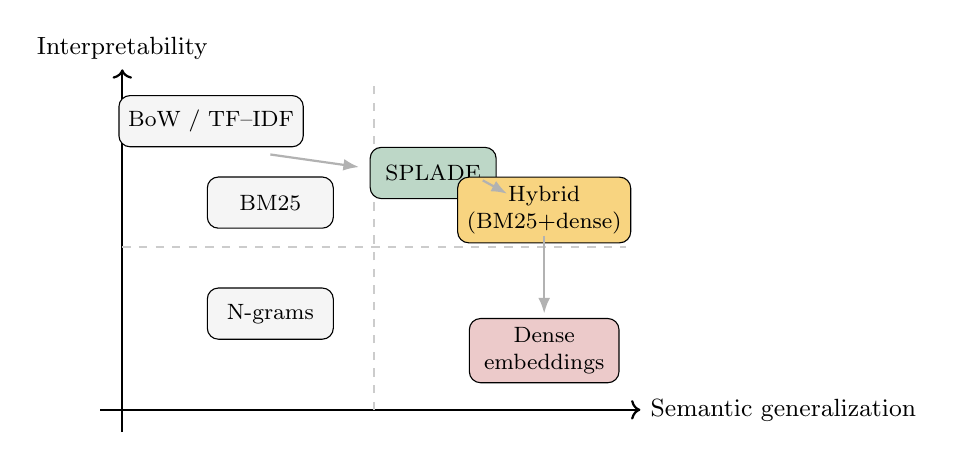
\begin{tikzpicture}[scale=0.94]
\draw[->,thick] (-0.3,0) -- (7.0,0)
    node[right,font=\small]{\small Semantic generalization};
\draw[->,thick] (0,-0.3) -- (0,4.6)
    node[above,font=\small]{\small Interpretability};
\draw[dashed,gray!40] (3.4,0)   -- (3.4,4.4);
\draw[dashed,gray!40] (0,2.2)   -- (6.8,2.2);
\node[draw,rounded corners,fill=SoftGray,font=\footnotesize,
    align=center,minimum width=1.9cm,minimum height=0.65cm] at (1.2,3.9){BoW / TF--IDF};
\node[draw,rounded corners,fill=SoftGray,font=\footnotesize,
    align=center,minimum width=1.6cm,minimum height=0.65cm] at (2.0,2.8){BM25};
\node[draw,rounded corners,fill=Forest!30,font=\footnotesize,
    align=center,minimum width=1.6cm,minimum height=0.65cm] at (4.2,3.2){SPLADE};
\node[draw,rounded corners,fill=Accent!50,font=\footnotesize,
    align=center,minimum width=1.9cm,minimum height=0.65cm] at (5.7,2.7){Hybrid\\(BM25+dense)};
\node[draw,rounded corners,fill=DeepRed!25,font=\footnotesize,
    align=center,minimum width=1.9cm,minimum height=0.65cm] at (5.7,0.8){Dense\\embeddings};
\node[draw,rounded corners,fill=SoftGray,font=\footnotesize,
    align=center,minimum width=1.6cm,minimum height=0.65cm] at (2.0,1.3){N-grams};
\draw[-{Latex[length=2mm]},gray!60,thick] (2.0,3.45) -- (3.2,3.28);
\draw[-{Latex[length=2mm]},gray!60,thick] (4.87,3.1) -- (5.2,2.92);
\draw[-{Latex[length=2mm]},gray!60,thick] (5.7,2.35) -- (5.7,1.3);
\end{tikzpicture}
\end{center}
\end{column}
\begin{column}{0.41\textwidth}
\vspace{0.2cm}
The sparse--dense axis is not a single staircase.
 
\vspace{0.2cm}
\begin{block}{Key takeaway}
SPLADE and hybrid retrieval occupy intermediate positions, combining the speed and
interpretability of sparse methods with the semantic reach of dense embeddings.
\end{block}
 
\vspace{0.15cm}
\begin{alertblock}{For the course}
Lessons~1--2 build the two extremes. Lesson~4 shows how they are combined in RAG pipelines.
\end{alertblock}
\end{column}
\end{columns}
\end{frame}
